\section{DATA AND DESCRIPTIVE ANALYSIS }

\begin{onehalfspace}
This section first provides a comprehensive overview of the data and
methodology used in the thesis. The primary dataset used throughout
the study comes from the Household Labor Force Surveys of (HLFS) TurkStat,
conforming to the standards set by the International Labor Organization
\citeyearpar{ILO2012}, with specific considerations for country-specific
comparability. The dataset encompasses the period from 2004 to 2022.
while changes in sampling design in 2004 and substantial alterations
in 2014 led to comparability concerns within the series.

The HLFS data uses a household-level yearly repeated cross-sectional
survey design. Key demographic variables such as education level,
monthly wage, occupation, economic sector, working hours, and years
of seniority in the current job are essential for our analysis. Given
that our aim is to scrutinize the structural shifts in labor force
dynamics over the past two decades, all available pertinent data is
valuable. Therefore, the data-cleaning approach drops the least number
of observations at each step as possible.

While the dataset provides samples starting from 2000, the comparability
of years prior to 2004 is compromised by substantial changes in the
sampling design which forces us to focus on the period between 2004
and 2022. Moreover, it is crucial to acknowledge that substantial
alterations were introduced in 2014 to ensure compliance with European
Union standards and accommodate new administrative divisions as mandated
by the Turkish government. These changes rendered the series incomparable
with prior data due to shifts in survey design and population projections,
as documented by TurkStat. While the repeated cross-sectional data
structure facilitates the investigation of time-varying relationships,
unity in sampling design becomes crucial. The modifications in 2014
restrict the feasibility of pooling observations from all available
periods within the dataset without making necessary arrangements.

A notable transformation within the dataset is attributed to a significant
change in education classification in 2014. From 2004 to 2013, education
levels were characterized based on the ISCED 1997 framework. Subsequently,
starting in 2013, the education classification shifted to the ISCED
2011 framework, providing more detailed delineation of the upper tiers
of educational segmentation \citep{OECD2015}.

In alignment with the International Labor Office's efforts to refine
classifications, TurkStat undertook transitions in occupational coding
systems, moving from ISCO68 to ISCO88 in 2004 and subsequently from
ISCO88 to ISCO08 in 2012. While ISCO68 and the data preceding 2004
displayed distinct structural characteristics, ISCO88 and ISCO08 are
more similar regarding occupational coding.

Despite minor changes between ISCO08 and ISCO88, ILO suggested that
authoritative institutes in countries should reorganize occupation
codes according to their unique labor market conditions \citep{ILO2012}.
Therefore, the major changes in occupation shares between 2011 and
2012 can be attributed to Turkey's adjustment procedure in switching
ISCO classifications.\footnote{A transition matrix provided with the 2012 Labor Force Survey data
package by TurkStat describes the switching process in numbers can
be found in Appendix}

The surge in service-oriented employment in 2012 amounted to approximately
one million jobs. Within this increment, 400,000 originated from the
managerial category, while an additional 300,000 came from elementary
occupations. A more detailed analysis of the shift from managerial
occupations to service jobs reveals that 68\% of the shifted observations
were self-employed, while 28\% were employers. This pattern highlights
a straightforward approach that TurkStat employed during the adoption
of the new ISCO classification.

According to ILO's report \citep{ILO2012} self-employed workers are
only classified as managers if their task at work primarily consists
of supervising staff. Otherwise, they are assigned to occupations
according to their primary tasks. Therefore it is reasonable to interpret
this shift as reflecting an increasing number of small firms in growing
service occupations that are coded as service jobs. The sectoral composition
of these jobs is strictly subjected to the wholesale and retail trade
of goods.

Table \ref{tab:Summary-Statistics-} shows summary statistics starting
from 2004 with four years intervals. To observe general trends, agricultural
workers are included in the table. These observations will be excluded
in the later phase, where the general trends of wage labor will be
analyzed through econometric methods. The aging speed of the labor
force, increasing firm sizes, and increasing service jobs can be observed
from the table at first glance. Notably, the share of workers with
a university degree in the workforce has tripled throughout the sample
period. The difference of average educational attainment for female
and male samples is plotted in Figure \ref{fig:Share-of-Hours}.

\begin{comment}
\begin{onehalfspace}
The summary statistics table, which consists of employed people, shows
that the education level has increased remarkably throughout the observed
period. While 14\% of the female labor force was illiterate in 2004,
this rate dropped to 4.6\% in 2021. In 2004, the rate of illiterate
female workforce was almost the same as the rate of university graduate
female labor force. However, by 2021, the rate of university-graduate
women in the labor force increased to 36\%. This rate fell from 2.4\%
in 2004 to less than 1\% for men in 2021. While the rate of university
graduate male workforce was 10.4\% in 2004, it increased to 24.8\%
in 2021. For women and men, half of the workforce had primary school
diploma or dropped out of primary school in 2004. This rate dropped
to 27\% in 2021. Overall, middle school or high school graduation,
which we consider the average in terms of years in education level,
accounts for half of the male workforce in 2021 while less than 30\%
in women. This situation causes the female workforce to become more
polarized regarding education level.
\end{onehalfspace}
\end{comment}

When comparing the years 2004 and 2022, an upward trend in the workforce's
average age becomes apparent. In 2004, 18.6\% of workers fell within
the age bracket of 15 to 24, declining to 14\% in 2022. This trend
could be attributed to a growing inclination among the youth to pursue
further education rather than entering the workforce early. As a result,
the labor force has witnessed increased educational attainment levels,
while the retirement age continues to rise.

In 2004, the proportion of females in the workforce stood at 25\%,
which expanded to a level of 32\% in 2022. A similar progression is
observed in the ratio of having social security. Despite these improvements,
there remains room for enhancement, particularly concerning issues
like pension entitlements and access to healthcare services. While
the prevalence of precarious employment has diminished, there has
been an escalation in part-time work rates, surging from 3.8\% to
18\%.

Consistent with other observed trends, there has been a decrease of
approximately 3 years in the average experience within current jobs.
Notably, a seemingly high proportion of workers, around 90\%, reported
their employment as permanent in 2004. However, this figure can be
misleading, as the starting point for this rate began at 55\% in 2008
and has exhibited a consistent upward trajectory thereafter. Moreover,
the presence of unpaid family workers and self-employed individuals
within the labor force experienced a decline of over 8\% over the
observed period. This trend was offset by the proportion of wage or
salaried employees, which reached 70\% by 2022.
\end{onehalfspace}
\begin{center}
\begin{table}[H]
\caption{\label{tab:Summary-Statistics-}Summary Statistics for Demographic
Variables}

\begin{centering}
\noindent\resizebox{\textwidth}{!}{%
\begin{tabular}{lr@{\extracolsep{0pt}.}lr@{\extracolsep{0pt}.}lr@{\extracolsep{0pt}.}lr@{\extracolsep{0pt}.}lr@{\extracolsep{0pt}.}l}
\toprule 
 & \multicolumn{2}{c}{2004} & \multicolumn{2}{c}{2008} & \multicolumn{2}{c}{2012} & \multicolumn{2}{c}{2016} & \multicolumn{2}{c}{2022}\tabularnewline
\midrule 
\textit{Education} & \multicolumn{2}{c}{} & \multicolumn{2}{c}{} & \multicolumn{2}{c}{} & \multicolumn{2}{c}{} & \multicolumn{2}{c}{}\tabularnewline
Below primary & 8&49\% & 7&9\% & 8&2\% & 6&3\% & 4&8\%\tabularnewline
Primary & 46&5\% & 39&4\% & 35&3\% & 30&95\% & 24&1\%\tabularnewline
Secondary & 12&8\% & 15&5\% & 17&7\% & 19&3\% & 17&9\%\tabularnewline
High school & 20&5\% & 22&1\% & 20&34\% & 20&6\% & 25&0\%\tabularnewline
University & 11&6\% & 15&1\% & 18&4\% & 22&7\% & 28&2\%\tabularnewline
\midrule 
\textit{Age Group} & \multicolumn{2}{c}{} & \multicolumn{2}{c}{} & \multicolumn{2}{c}{} & \multicolumn{2}{c}{} & \multicolumn{2}{c}{}\tabularnewline
15-24 & 18&6\% & 16&9\% & 15&1\% & 15&3\% & 14&2\%\tabularnewline
25-34 & 31&9\% & 32&5\% & 31&3\% & 28&6\% & 26&4\%\tabularnewline
35-44 & 27&3\% & 27&4\% & 27&8\% & 28&7\% & 28&5\%\tabularnewline
45-54 & 15&7\% & 16&7\% & 18&0\% & 18&8\% & 20&9\%\tabularnewline
55-64 & 6&5\% & 6&5\% & 7&7\% & 8&7\% & 10&0\%\tabularnewline
\midrule 
Female & 25&5\% & 26&4\% & 29&4\% & 30&7\% & 32&5\%\tabularnewline
Married & 74&1\% & 73&4\% & 72&1\% & 70&0\% & 66&2\%\tabularnewline
Having social security & 51&1\% & 57&8\% & 62&2\% & 67&9\% & 75&0\%\tabularnewline
Permanency of job & 89&5\% & 55&5\% & 56&6\% & 59&9\% & 64&5\%\tabularnewline
Having additional job & 2&1\% & 2&6\% & 3&0\% & 3&3\% & 2&6\%\tabularnewline
Part time worker ratio & 3&8\% & 12&0\% & 18&5\% & 17&5\% & 18&4\%\tabularnewline
Average tenure in job & 12&2 & 10&2 & 9&4 & 9&7 & 9&5\tabularnewline
\midrule 
\textit{Employment Status} & \multicolumn{2}{c}{} & \multicolumn{2}{c}{} & \multicolumn{2}{c}{} & \multicolumn{2}{c}{} & \multicolumn{2}{c}{}\tabularnewline
Wage or salaried employee & 54&6\% & 61&0\% & 62&9\% & 67&6\% & 70&5\%\tabularnewline
Employer & 5&1\% & 5&9\% & 5&0\% & 4&6\% & 4&5\%\tabularnewline
Self employed & 23&3\% & 20&4\% & 18&9\% & 16&7\% & 16&3\%\tabularnewline
Unpaid family worker & 17&0\% & 12&7\% & 13&2\% & 11&2\% & 8&7\%\tabularnewline
\midrule 
\textit{Firm Size} & \multicolumn{2}{c}{} & \multicolumn{2}{c}{} & \multicolumn{2}{c}{} & \multicolumn{2}{c}{} & \multicolumn{2}{c}{}\tabularnewline
<10 & 62&6\% & 57&5\% & 56&2\% & 54&2\% & 47&1\%\tabularnewline
10 to 50 & 16&6\% & 20&2\% & 21&3\% & 19&8\% & 23&7\%\tabularnewline
50 or more & 20&6\% & 22&31\% & 22&2\% & 25&8\% & 29&1\%\tabularnewline
Don't know but more than 10 & \multicolumn{2}{c}{0} & \multicolumn{2}{c}{0} & \multicolumn{2}{c}{0} & 0&1\% & 0&1\%\tabularnewline
\midrule 
\textit{Workplace Type} & \multicolumn{2}{c}{} & \multicolumn{2}{c}{} & \multicolumn{2}{c}{} & \multicolumn{2}{c}{} & \multicolumn{2}{c}{}\tabularnewline
Field, garden & 31&4\% & 24&9\% & 26&2\% & 20&6\% & 16&6\%\tabularnewline
Regular & 56&6\% & 65&7\% & 63&9\% & 69&1\% & 72&6\%\tabularnewline
Market place & 1&1\% & 0&8\% & 0&6\% & 0&6\% & 0&6\%\tabularnewline
Mobile or irregular & 9&4\% & 7&3\% & 7&0\% & 7&01\% & 5&6\%\tabularnewline
At home & 1&5\% & 1&3\% & 2&2\% & 2&6\% & 4&6\%\tabularnewline
\midrule 
Number of observations & \multicolumn{2}{c}{131,389} & \multicolumn{2}{c}{135,250} & \multicolumn{2}{c}{159,424} & \multicolumn{2}{c}{164,130} & \multicolumn{2}{c}{211,536}\tabularnewline
\bottomrule
\end{tabular}}
\par\end{centering}
\medskip{}

\textbf{Notes: }The table displays changes in the demographics of
the employed workforce between the ages of 15 and 64 over the data
period. The values in the table may not sum up to 100 due to truncation.
\end{table}

\par\end{center}

\begin{center}
\begin{table}[H]
\caption{\label{tab:Summary-Statistics-occupations}Summary Statistics for
Occupation Categories and Economic Sectors}

\begin{centering}
\noindent\resizebox{\textwidth}{!}{%
\begin{tabular}{lr@{\extracolsep{0pt}.}lr@{\extracolsep{0pt}.}lr@{\extracolsep{0pt}.}lr@{\extracolsep{0pt}.}lr@{\extracolsep{0pt}.}l}
\toprule 
 & \multicolumn{2}{c}{2004} & \multicolumn{2}{c}{2008} & \multicolumn{2}{c}{2012} & \multicolumn{2}{c}{2016} & \multicolumn{2}{c}{2022}\tabularnewline
\midrule 
\textit{Occupation} & \multicolumn{2}{c}{} & \multicolumn{2}{c}{} & \multicolumn{2}{c}{} & \multicolumn{2}{c}{} & \multicolumn{2}{c}{}\tabularnewline
Managers & 9&2\% & 8&8\% & 7&7\% & 5&2\% & 5&5\%\tabularnewline
Professionals & 6&8\% & 6&4\% & 7&9\% & 10&4\% & 12&4\%\tabularnewline
Technicians & 5&6\% & 7&3\% & 6&5\% & 5&7\% & 6&6\%\tabularnewline
Clerks & 5&9\% & 6&8\% & 7&2\% & 7&3\% & 7&2\%\tabularnewline
Service and sales & 11&0\% & 12&1\% & 13&0\% & 19&0\% & 19&5\%\tabularnewline
Agriculture & 23&3\% & 17&9\% & 18&1\% & 13&5\% & 10&4\%\tabularnewline
Craft and related trade & 15&1\% & 14&6\% & 13&2\% & 13&8\% & 13&1\%\tabularnewline
Machine operators & 10&6\% & 11&0\% & 10&5\% & 9&5\% & 9&9\%\tabularnewline
Elementary & 12&4\% & 14&9\% & 15&8\% & 15&5\% & 15&4\%\tabularnewline
\midrule 
\textit{Sector} & \multicolumn{2}{c}{} & \multicolumn{2}{c}{} & \multicolumn{2}{c}{} & \multicolumn{2}{c}{} & \multicolumn{2}{c}{}\tabularnewline
Agriculture & 27&1\% & 22&1\% & 23&1\% & 18&0\% & 14&4\%\tabularnewline
Manufacturing and mining & 20&6\% & 21&4\% & 19&5\% & 19&8\% & 22&1\%\tabularnewline
Construction & 5&0\% & 6&0\% & 7&0\% & 7&4\% & 6&1\%\tabularnewline
Trade and transportation & 21&0\% & 21&3\% & 18&8\% & 18&4\% & 19&3\%\tabularnewline
Accommodation and food services & 4&2\% & 4&8\% & 5&0\% & 5&5\% & 5&6\%\tabularnewline
Information and communication & 0&8\% & 0&8\% & 0&9\% & 0&94\% & 0&9\%\tabularnewline
Finance, insurance and real estate & 1&5\% & 1&5\% & 1&8\% & 2&0\% & 2&1\%\tabularnewline
Community, personal and other services & 19&6\% & 22&0\% & 23&7\% & 27&7\% & 29&4\%\tabularnewline
\midrule 
Number of observations & \multicolumn{2}{c}{131,389} & \multicolumn{2}{c}{135,250} & \multicolumn{2}{c}{159,424} & \multicolumn{2}{c}{164,130} & \multicolumn{2}{c}{211,536}\tabularnewline
\bottomrule
\end{tabular}}
\par\end{centering}
\medskip{}

\textbf{Notes: }The table displays changes in the demographics of
the employed workforce between the ages of 15 and 64 over the data
period. The values in the table may not sum up to 100 due to truncation.
\end{table}

\par\end{center}

\vspace{-1cm}

\begin{onehalfspace}
Table \ref{tab:Summary-Statistics-occupations}, shows substantial
differences in occupations' share throughout the observed period.
After a steady decline in the share of managers in the first period
(2004--2012), their share dropped 2.5\% in 2016 and stayed relatively
stagnant after. Conversely, the proportion of professionals began
ascending after 2008, displaying a relatively steady growth rate and
reaching 12.4\% in 2022. Meanwhile, technicians' share surged to 7.3\%
in 2008 and stayed more or less the same in the following period.

The workforce underwent its most significant transformation in the
services and sales jobs, as well as in the proportion of agricultural
workers. The proportion of agricultural workers, which once constituted
nearly a quarter of the workforce, declined to 10.4\% by 2022. In
stark contrast, the relative size of services and sales jobs doubled,
surging to 19.5\% in the same year. Elementary jobs experienced a
notable increase of over 3\% in their share in 2012, sustained at
that level after that.

Analyzing the sectoral distribution of the workforce, the community,
personal, and other services sector exhibited a growth of 10\% over
the observed period. Conversely, a similar declining trend was observed
in the sectoral share of agriculture, mirroring the pattern seen in
the occupational share of agriculture. Particularly noteworthy is
the continuous increase in the construction sector's share until 2016,
after which a decline of 1.5\% was witnessed over the subsequent 6
years.

The change in firm size parallels the change in the self-employed
workforce. When considered together with the increase in the number
of chain stores, the 17-year change in the Turkish workforce shows
that self-employed artisans and those working in the agricultural
sector with irregular income have shifted to jobs for which they receive
regular wages over time.
\end{onehalfspace}
\begin{center}
\begin{figure}[H]
\caption{\label{fig:Share-of-Hours}Share of Hours Worked by Education and
Gender}

\begin{centering}
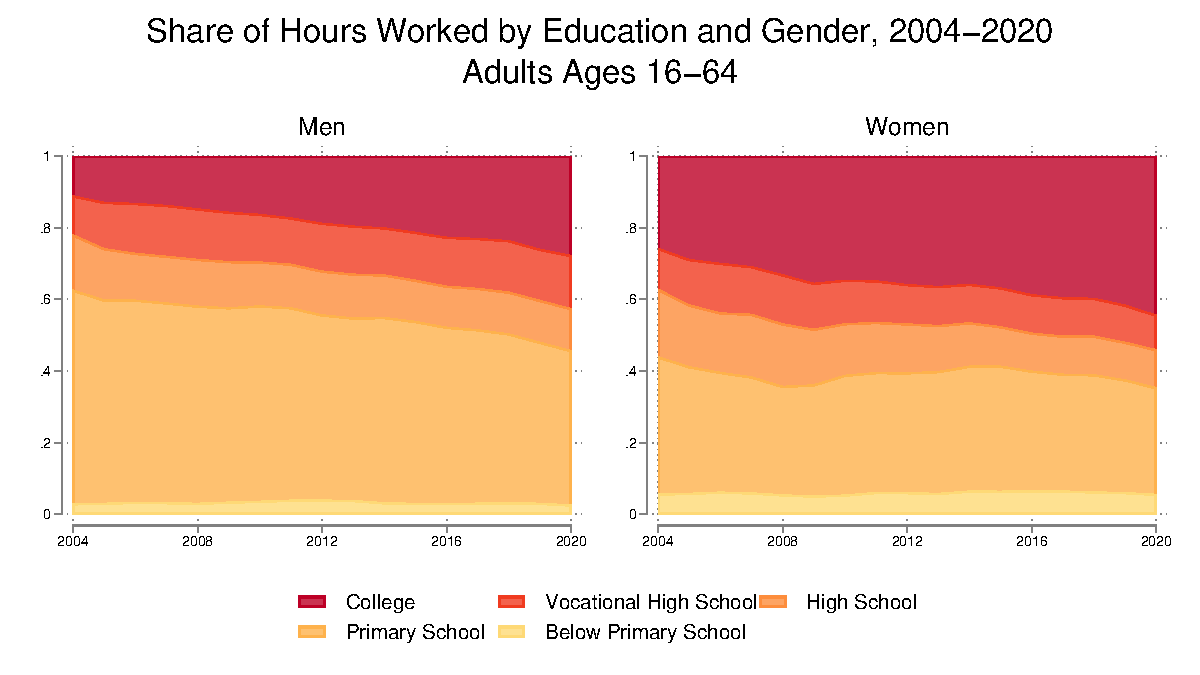
\includegraphics[width=1\textwidth]{figs/ch2/educ-hour-shares-mf-2004-2020.pdf}
\par\end{centering}
\medskip

\begin{singlespace}
\textbf{Source:} Author's calculations based on HLFS, following the
framework used by \citet{Autor2019}.
\end{singlespace}
\end{figure}
\par\end{center}

\vspace{-1cm}

\begin{onehalfspace}
There is a different structure in Figure \ref{fig:Share-of-Hours}.
To observe labor market trends systematically, we focused solely on
wage or casual employees working full-time, as hourly wage data provides
a Because, we aim to observe the labor market trends in a more systematic
way and hourly wage data provides a convenient tool for this purpose.
In creating a consistent sample of hourly wages, we set certain restrictions,
including excluding part-time workers. Following \citet{2019Autor},
labor supply weights were calculated based on each worker's usual
weekly earnings. As a result, the relationship between the total hours
worked by wage earners and their education level from 2004 to 2020
has been shown. Similar to Table 1, a secular increase was observed
in the share of employees with undergraduate and graduate degrees,
including two-year departments. However, we encountered a limitation
due to changes in education-level coding as of 2008. Before 2008,
a negligible part of the workforce held master's or doctoral degrees,
but after 2008, they were included in the dataset with separate coding
as their share increased. To ensure comparability with the pre-2008
dataset, we considered employees with master's and doctoral degrees
as university graduates.
\end{onehalfspace}

\subsection{Turkey's Labor Market Trends}

\begin{onehalfspace}
In this subsection, we visualize the data set to identify labor market
trends using well-studied methods in line with the literature. Firstly,
we use the pioneering frame work of KM, which inspired many studies
from various regions of the World, including \citet{2015Bakis,RePEc:erg:wpaper:1509}.

KM utilized a supply and demand framework to analyze changes in relative
workers for different skill groups. They created two separate samples:
one for measuring labor supply (count sample) and the other for measuring
wages (wage sample). The wage sample aimed to maintain a relatively
constant composition over time, focusing on full-time workers who
are less likely to leave the labor force. On the other hand, the count
sample included all workers, including part-time employees, to measure
aggregate labor output.
\end{onehalfspace}

\begin{onehalfspace}
We start by applying the supply and demand framework to Turkey to
decompose the wage structure. Following KM and AA, and \citet{2015Bakis},
each wave of dataset is transformed in a way to form two samples,
one of which is comprising wages and the other has the quantity of
labor supplied. In order to assess the impact of labor supplied by
the workers and the relative wages, the wage sample is used to determine
the wage index and the count sample is used to calculate the hours
of labor work for each demographic group. Demographic groups are cells
that represent the labor force with the most dimensions possible.
There are five education categories, which are: below 8 years of educational
attainment, primary school (8 years), high school (11 years), vocational
high school (12 years), and university (15+)\footnote{After, 2014's cross-section, the university graduates are separated
into further categories. But we collapsed them into one major category
of college education to maintain comparability with the previous years.
More detail about the treatment on data can be found in Data Appendix.}. Experience is also categorized into five groups. In similar studies,
experience cells have ten years intervals (0-9, 10-19, 20, 29...).
However there are several shortcomings stemming from that, such as
obtaining no or too few observations for a couple of cells. To overcome
this shortcoming, the following form of categorization is used instead
of ten years of equal intervals in this study: 0-5 years, 6-10 years,
11-15, 16-20, 21-48.
\end{onehalfspace}
\begin{onehalfspace}
\begin{center}
$x_{new}$=$\begin{cases}
2, & if\ x\leqq5\\
7, & if\ 6\leqq x\leqq10\\
13, & if\ 11\leqq x\leqq15\\
17, & if\ 16\leqq x\leqq20\\
30, & if\ 21\leqq x\leqq48
\end{cases}$
\par\end{center}
\end{onehalfspace}

\begin{onehalfspace}
where $x_{new}$ stands for the new experience categories created
and $x$ is the experience levels reported by respondents.

Unlike \citet{2015Bakis}, after achieving a full working sample,
log hourly and weekly wages for all observations are regressed on
five education dummies, a quartic in experience, interactions of quartic
in experience with education and gender dummies, and a dummy of part-time
workers. After predicting log weekly and hourly wages for each series,
wages are deflated by using GDP deflators. Than, we collapse the predicted
log real wages into cells. Therefore, we achieve a sample of 50 observations
(N = 50) consisting of education-experience-gender cells for each
wave. Taking into account the assumptions of the supply and demand
framework, the self employed labor and unpaid family workers are excluded.
Because, aside from these two categories, our framework is based on
the assumption that wage levels are signaling the comparative advantage
of different endowments in the labor market.

There are $N_{k}$ observations in each of the $k$ cells representing
the labor input. A wage-supply index is calculated for each cell $k$.
In order to measure the effect of labor supply on the wage levels,
the approach we follow is to create constant compositions of labor
which can be followed throughout the whole period in the data set
(2004 to 2020). Thus the computed wage index follows a \emph{composition
adjusted} form while the supply index helps us measure the aggregate
labor supply over time.

Computation of the wage cell is given by:%
\begin{comment}
\begin{onehalfspace}
\begin{center}
$W_{k}=\dfrac{\sum_{i=1}^{N_{k}}{\lambda_{ik}w_{ik}}}{\sum_{i=1}^{N_{k}}{\lambda_{ik}h_{ik}}}, k=1,2,...,N,$
\par\end{center}
\end{onehalfspace}
\end{comment}
\[
W_{k}=\dfrac{\sum_{i=1}^{N_{k}}{\lambda_{ik}w_{ik}}}{\sum_{i=1}^{N_{k}}{\lambda_{ik}h_{ik}}},k=1,2,...,N
\]

\end{onehalfspace}

\begin{onehalfspace}
\emph{$\lambda_{ik}$} stands for the sample weights, $w_{ik}$ and
$h_{ik}$ represents real wage and working hours, respectively. We
formed a matrix of \emph{N x T, }showing hourly wage of each cell
we created for demographic variables.

To create a \emph{count sample}, the total labor supply measured by
usual weekly working hours in each cell is computed using sampling
weights for each observation. To obtain a relative supply index, a
transformation is conducted for the sample of quantities to calculate
shares of each cell by dividing the total hours worked in each cell
by the total hours worked over all cells in the economy to get the
employment share of each cell.

To facilitate our analysis of wage premiums for education levels,
we calculate the measure called \emph{efficiency units. }Using a \emph{fixed
wage }approach, we first computed the average relative wage for each
cell. However, since the skill levels within a broad category is not
homogeneously distributed, taking the average of labor supply within
a category would not be an accurate measure because it does not account
for the experience levels. In order to measure relative efficiencies
in terms of labor for workers whose experience levels are different
from each other, we need to deflate the aggregate wage of a cell with
the reference wage. The relative wage of cell $k$, $z_{k}$, is obtained
by subtracting the aggregate wage of cell $k$ from the value of the
reference wage selected for that year. The \emph{N x T} matrix, abbreviated
as \emph{Z}, represents the average yearly wages across all demographic
groups. Our \emph{efficiency units} are the mean values of these relative
wages, \emph{Z} (an N-element column vector), over the years.\footnote{In this case, we created two broad categories to see college premium:
college graduates and non-college graduates. The reference wage is
set to the max wage of a male with high school diploma and ten years
of experience.} After creating a matrix of\emph{ }efficiency units, we use them to
create aggregate supply indexes. First, the product of efficiency
units with labor supply of the cell is computed for males and females.
Than the fixed wage of the same cell is used to get the efficient
labor supply of cell k (\emph{Ek = }$h_kz_k$). We next create aggregate
supply indexes (again in efficiency units) for further aggregate groups
using these efficiency units. The total supply of efficient labor
is then calculated by adding up all groups, resulting in Z0H (a T-element
row vector). We obtain E, a \emph{N x T} matrix made up of relative
supplies (measured in efficiency units) of all demographic groups
for each year, by deflating the efficient labor supply of each cell
by the corresponding total efficient labor supply. Finally, we obtain
efficient labor supply indices for these broad categories by summing
over the sub-cells constituting them (for instance, skilled/unskilled).
\citep{2008Autor}

The wage indexes for broad categories, such as college graduates,
are calculated using a f\emph{ixed-weight} methodology. The aggregate
wage for each category, denoted as \emph{L} (an \emph{N}-element column
vector), is computed as the raw employment share weighted by arithmetic
means. This approach allows us to control for factors affecting the
wage level in our category of interest. These aggregates are referred
to as These aggregates are known as \emph{composition adjusted} or
composition constant aggregates, as they maintain the composition
of major education categories over time, thus controlling for compositional
changes. By making this adjustment, we ensure that shifts do not influence
the estimated college premium in other controlled factors, such as
gender composition, level of experience, or level of educational attainment
within the categories of college graduates and non-college graduates.

After 2010, increase in the college premium is stopped which can be
seen in \ref{fig:College-High-School-Wage-fig3}, but it's sharp decline
started after 2014. A college premium of 41 log points implies that,
in 2004, the earnings of an average college graduate were 50 percent
higher (i.e., exp(0.41) -- 1$\simeq$ 0.50) than the average wage
of a worker without college diploma. After reaching its initial level
around 2017, the college premium remained around 44 percent in 2020
We present a different form of figure \ref{fig:College-High-School-Wage-fig3}.
Figure \ref{fig:College-High-School-Experience} in the Appendix shows the picture of two different experience
cohorts.

College premium, which can be considered as the valuation of skills
determined trough the market forces, is linked to it's supply, among
other factors. While figure \ref{fig:Composition-Adjusted-College/Hig-wage}
depicts the premium of education, figure \ref{fig:Comosition-adjustedCollege/High-School-supply}
is showing the situation in terms of labor supplied by each educational
level.
\end{onehalfspace}
\begin{onehalfspace}
\begin{center}
\begin{figure}[H]
\begin{centering}
\caption{\label{fig:College-High-School-Wage-fig3}College-High-School Wage
and Supply Dynamics, 2004-2020}
\par\end{centering}
\begin{centering}
\subfloat[\label{fig:Composition-Adjusted-College/Hig-wage}Composition Adjusted
College/High-School Log Real Weekly Wages Ratio, 2004-2020]{\begin{centering}
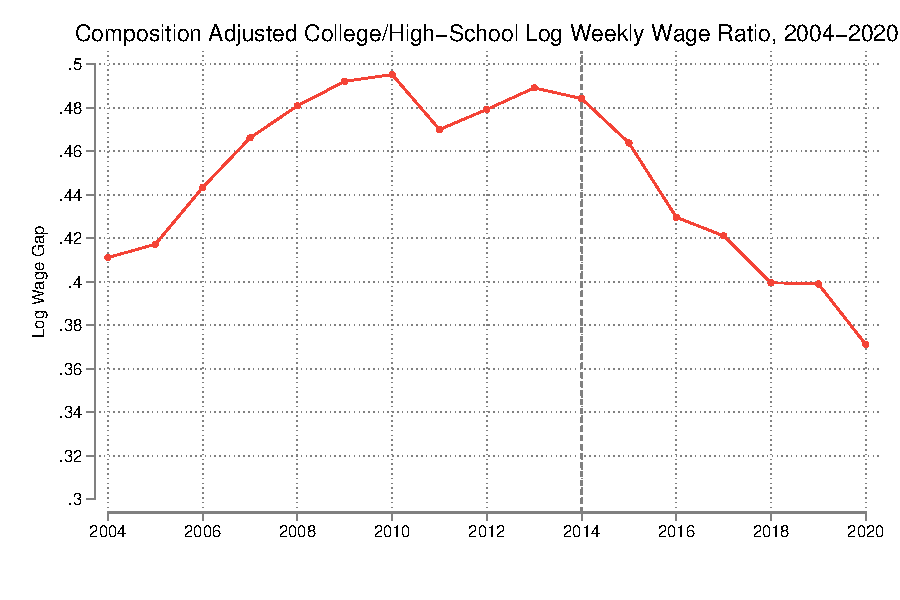
\includegraphics[width=0.6\paperwidth]{figs/ch2/college-hs-wage-premium-comp-adj.pdf}
\par\end{centering}
}
\par\end{centering}
\begin{centering}
\subfloat[\label{fig:Comosition-adjustedCollege/High-School-supply}College/High-School
Log Relative Supply, 2004-2020]{\centering{}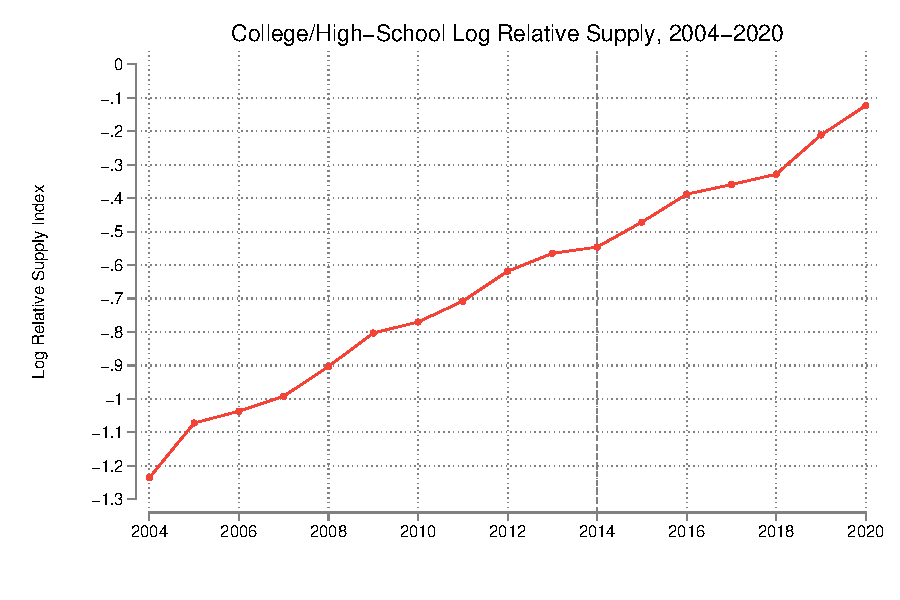
\includegraphics[width=0.6\paperwidth]{figs/ch2/college-hs-relative-supply-comp-adj.pdf}}
\par\end{centering}
\medskip

\begin{singlespace}
\textbf{Source:} Author's calculations by using efficiency units.
\end{singlespace}
\end{figure}
\par\end{center}
\end{onehalfspace}

\vspace{-1cm}

\begin{onehalfspace}
Growth in the level of college graduates shows a secular form, reaching
to almost half of the work force in 2020. Initial level of relative
labor supply was three college graduates for every ten worker who
did not complete or attend to any college eduction. A different version
of Figure \ref{fig:Composition-Adjusted-Educ-Cohorts-1} is presented
individual plots of female and male data is presented in Appendix
Figure \ref{fig:Composition-Adjusted-Educ-Cohorts-2}.
\end{onehalfspace}
\begin{onehalfspace}
\begin{center}
\begin{figure}[H]
\begin{singlespace}
\caption{\label{fig:Composition-Adjusted-Educ-Cohorts-1}Composition Adjusted
Log Real Wages of Education Cohorts (2004-2020)}

\end{singlespace}
\begin{centering}
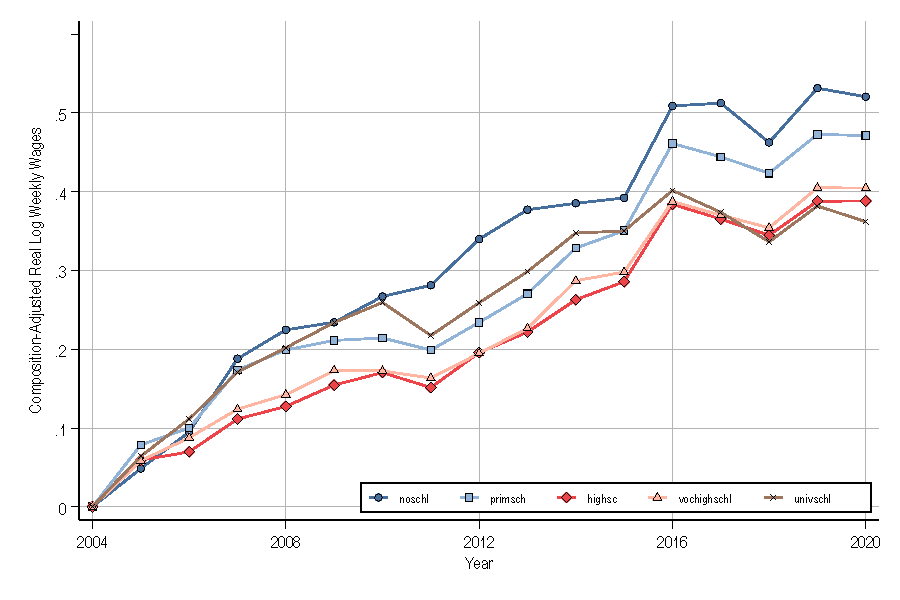
\includegraphics[width=1\textwidth]{figs/ch2/comp-adj-log-wages-mf-2004-2020.pdf}
\par\end{centering}
\medskip

\begin{singlespace}
\textbf{Source: }Authors's calculatiıons using HLFS (2004-2020).
Calculation of the labor supply is based on the reported usual weekly
working hours of all persons aged 14-64 who are employed and either
recieving a monthly wage or a salary. The real log weekly wages for
each education category is the weighted average of the relevant composition
adjusted cells using a fixed set of weights equal to the average employment
share of each group. Predicted nominal wages are deflated by the GDP
deflator. (noschl: below primary school, primsch: primary school,
highsc: high school, vochighschl: vocational high school, univschl:
college)
\end{singlespace}
\end{figure}
\par\end{center}
\end{onehalfspace}

\vspace{-1cm}

\begin{onehalfspace}
Wage premium predictions give little information on the real wage
levels of different skill groups. Declining college premiums might
be explained by a faster rise in non-college wages. Together with
the steady growth of the labor force holding a college diploma, growth
speed of college graduated labor force's wage levels stayed relatively
low, as we see in the figure \ref{fig:College-High-School-Wage-fig3}.
Moreover, Figure \ref{fig:Composition-Adjusted-Educ-Cohorts-2}, gives
more detailed information on real earnings of five education groups
and two gender groups. Figure plots the evolution of log wages throughout
the period under study. Each series is normalized to zero in the beginning
year. Values are corresponded to the log changes of wages relative
to it's initial level, which is 2004. Starting from the beginning
years, wage increases for workers with primary school diplomas and
below are faster than for high school graduates. Although college-graduated
workers' wage increases align with the unskilled labor for the first
5 years, their wage levels stagnated after 2014.
\end{onehalfspace}
\begin{center}
\begin{figure}[H]
\begin{singlespace}
\caption{Cumulative Log Real Wage Growth at the 90th, 50th and 10th Wage Percentiles
(2004-2020)}

\end{singlespace}
\begin{centering}
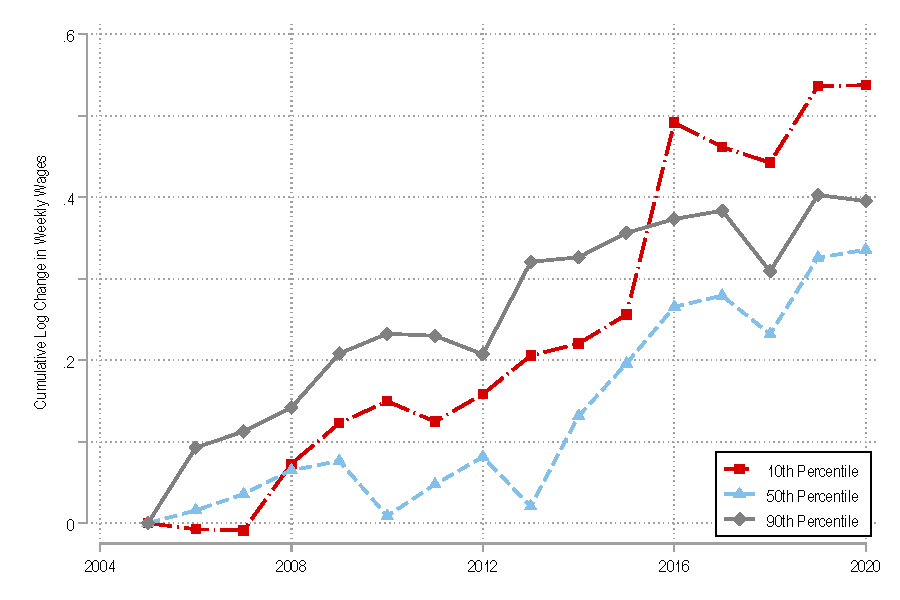
\includegraphics[width=1\textwidth]{figs/ch2/wage-percentiles-90-50-10-mf.pdf}
\par\end{centering}
\begin{singlespace}
\medskip
\end{singlespace}

\begin{singlespace}
\textbf{Source:} Labor Force Survey cross-sections from 2004 to 2020
are pooled. Similar to \citep{icsik2020heterogeneous} the sample
data cleaned to obtain full-time workers who have permanent jobs and
are earning more than 75\% of minimum wage for each particular year.
\end{singlespace}
\end{figure}
\par\end{center}

\vspace{-1cm}

\subsection{Shift-share Decomposition}

\begin{onehalfspace}
An indispensable explanation for the phenomenon of employment polarization
asserts that the configuration of industries has undergone a transformation,
gravitating towards economic sectors that exhibit diminished reliance
on ``routine'' occupations, while concurrently
embracing a greater reliance on ``abstract''
and ``manual'' tasks. To see if this explanation
fits into Turkish labor market, we use a shift share decomposition
method with a standard form, in line with the literature \citep{Acemoglu2011,2018Barany,2014Goos}.
The overall change in employment distribution of each occupation \textit{j,}
between year 0 and \textit{t} can be expressed as:
\begin{gather}
\varDelta E_{jt}=\sum_{k}\varDelta E_{kt}\lambda_{jk}+\sum_{j}\varDelta\lambda_{jkt}E_{k}\nonumber \\
\equiv\varDelta E_{t}^{B}+\varDelta E_{t}^{W},\label{eq:}
\end{gather}

Herein, $\varDelta E_{jt}$ denotes the change in the overall share
of employment in occupation \textit{j }over time period \textit{t}.
$\varDelta E_{t}^{B}$denotes the change in the share of employment
in occupation \textit{j }which is attributed to alterations in industrial
composition. The term $\varDelta E_{t}^{W}$ denotes variations in
the employment proportion of occupation \textit{j,} corresponding
to shifts occurring within-industries. $\varDelta E_{kt}=E_{kt_{1}}-E_{kt_{0}}$represents
the change in industry \emph{k}'s employment share during time \emph{t}.
$E_{kt}=(E_{kt_{1}}+E_{kt_{0}})/2$ is the mean employment distribution
of industry\emph{ k} across time span \emph{t} of four years. $\varDelta\lambda_{kt}=\lambda_{kt_{1}}-\lambda_{kt_{0}}$
quantifies the change linked to the occupation \emph{j}'s share employment
in industry \emph{k} over the specified time interval \emph{t}, and
$\lambda_{jkt}=(\lambda_{jkt_{1}}+\lambda_{jkt_{0}})/2$ represents
the average employment distribution of occupation \emph{j} within
industry \emph{k} during time \emph{t}.

In Table \ref{tab:Decomposition-of-Changes} we summarize the results.
First four columns splits the observation period into four equal segments,
followed by subsequent column showing the results for the extended
time period. Evidently, there is a clear pattern of occupational employment
share shifting towards Clerical and Managerial occupations, and elementary
occupations from occupations in manufacturing. This is in line with
RBTC hypothesis which posits a transfer of employment share towards
more skilled and less skilled occupations from middle skilled occupations.

The sharp rise in the employment share of clerical, administrative
and sales occupations during the interval of 2012-2016, was primarily
accounted for by the growth in employment within industries. This
change can be attributed to the adaptation process undertaken by TurkStat,
leading to the introduction of new occupational classifications in
2012. Notably, workers previously categorized as managers in small
enterprises (ISCO 13) transformed, transitioning to roles such as
salespersons and demonstrators, which are classified as ISCO 53 within
the updated occupational coding system. A corollary observation is
discernible in the reduction of total employment within non-routine
cognitive occupations, a shift predominantly explicable by changes
occurring within industries. This indicates that the workers previously
designated as managers, subsequently transitioned to sales jobs as
a direct outcome of the aforementioned coding transition.

The decline in blue collar routine manual jobs was counterbalanced
by the increase in clerical and elementary jobs within the aggregate
employment distribution. Notably, one third of the reduction in blue-collar
jobs can be attributed to the inter-industrial shift of workforce
allocation, primarily towards the service sector. It is noteworthy
that this inter-industrial redistribution has exhibited a gradual
deceleration over the past decade. Within industry component accounts
for fifty percent of the transformation observed in elementary jobs.
This implies that the augmentation in the overall employment share
within sectors that exhibit a demand for unskilled labor has been
responsible for half of the employment variation.
\end{onehalfspace}
\begin{center}
\begin{table}[H]
\caption{\label{tab:Decomposition-of-Changes}Decomposition of Changes in Terms
of Employment Shares in Broad Occupational Categories}

\begin{centering}
\begin{tabular}{l>{\raggedleft}p{0.55cm}@{\extracolsep{0pt}.}p{0.55cm}>{\raggedleft}p{0.55cm}@{\extracolsep{0pt}.}p{0.55cm}>{\raggedleft}p{0.55cm}@{\extracolsep{0pt}.}p{0.55cm}>{\raggedleft}p{0.55cm}@{\extracolsep{0pt}.}p{0.55cm}>{\raggedleft}p{0.55cm}@{\extracolsep{0pt}.}p{0.55cm}}
\toprule 
 & \multicolumn{2}{p{1.1cm}}{2004-2008} & \multicolumn{2}{p{1.1cm}}{2008-2012} & \multicolumn{2}{p{1.1cm}}{2012-2016} & \multicolumn{2}{p{1.1cm}}{2016-2022} & \multicolumn{2}{p{1.1cm}}{\textbf{Total}}\tabularnewline
\midrule 
\multicolumn{11}{l}{Professional, Managerial, and Technical Occs. (non-routine cognitive)}\tabularnewline
Total $\varDelta$ & 0&75 & -0&91 & -2&75 & 2&53 & -0&09\tabularnewline
Between $\varDelta$ & 0&20 & -0&18 & 0&17 & 0&24 & 0&11\tabularnewline
Within $\varDelta$ & 0&55 & -0&73 & -2&93 & 2&29 & -0&20\tabularnewline
\multicolumn{11}{l}{Clerical, Administrative and Sales Occs (routine cognitive)}\tabularnewline
Total $\varDelta$ & 1&08 & 0&30 & 5&33 & -0&65 & 1&51\tabularnewline
Between $\varDelta$ & 0&23 & 0&21 & 0&40 & 0&34 & 0&30\tabularnewline
Within $\varDelta$ & 0&84 & 0&08 & 4&93 & -0&99 & 1&21\tabularnewline
\multicolumn{11}{l}{Production, Craft, Repair and Operative Occs (routine manual)}\tabularnewline
Total $\varDelta$ & -3&38 & -1&71 & -2&74 & -1&38 & -2&30\tabularnewline
Between $\varDelta$ & -0&09 & -2&55 & -0&82 & -0&01 & -0&87\tabularnewline
Within $\varDelta$ & -3&28 & 0&84 & -1&91 & -1&37 & -1&43\tabularnewline
\multicolumn{11}{l}{Elementary (non-routine manual)}\tabularnewline
Total $\varDelta$ & 1&54 & 2&32 & 0&15 & -0&49 & 0&88\tabularnewline
Between $\varDelta$ & 0&6 & -0&33 & -0&00 & 0&10 & 0&46\tabularnewline
Within $\varDelta$ & -0&16 & -0&06 & -0&35 & 0&27 & 0&42\tabularnewline
\bottomrule
\end{tabular}
\par\end{centering}
\medskip

\textbf{Source:} Labor Force Surveys of 2004, 2008, 2012 and 2022.
Each set of three rows (Total, Industry, Occupation) shows the changes
in employment shares in four broad occupational categories, which
are constructed according to their principal task content. Time intervals
divide the study period into four equal periods. With this structure,
changes in employment shares decomposed into between and within-industry
components. The decomposition uses 8 broad occupational categories
(agricultural workers are excluded from the sample) and 17 broad industry
category. These groups are harmonized accordingly to obtain a full
sample. We do not impose any exclusion criteria, except for the omission
of part-time workers. This decision is based on the heterogenous presence
of non-permanent workers and individuals earning wages below the monthly
minimum wage level across occupation categories.
\end{table}

\par\end{center}

\vspace{-1cm}

\begin{onehalfspace}
\citet[hereafter, GM]{2014Goos} argue that the SBTC literature almost
entirely relies on the within-industry component on explaining skill
upgrading. However, between-industry component of employment changes
can be driven by routinization. Because, routinization is more substantially
impacts industries of routine occupations and displaces labor towards
other industries. Therefore, according to GM, RBTC will cause a between-industry
shift in blue-collar occupations. Despite the substantial effect of
between industrial shifts coming from the previously mentioned transition
process, about one third of the total shift can be attributed to change
in industrial composition.

Table \ref{tab:Changes-in-the-Shares-of-Hours-Worked} documents the
analysis similar to what is shown in table \ref{tab:Decomposition-of-Changes},
but with a different structure used by GM. They mapped the Routine
Task Intensity Index from \citet{2013Autor} to occupational classification
used by European countries. According to their mapping, the most routine
intensive occupation is office clerks (ISCO 41), while the least routine
intensive occupational category is managers of small enterprises (ISCO
13). In column 3 of table \ref{tab:Changes-in-the-Shares-of-Hours-Worked}
their RTI index is reported. For 21 occupations ranked by their mean
wage in 2004 (a broadly used proxy for skill level), column 1 and
column 2 presents average share of employment in 2004 and employment
change from 2004 to 2012, respectively. GM reported a substantial
decline in middle paying occupations and a substantial rise in high
paying and low paying occupations. Table \ref{tab:Changes-in-the-Shares-of-Hours-Worked}
presents some contrary trends in average employment shares. While
middle paying occupations and high paying occupations experienced
substantial employment growth in the time period, low paying occupations
accounts for all the growth in other sectors with a \%10 decline in
employment share.
\end{onehalfspace}
\begin{center}
\begin{table}[H]
\caption{\label{tab:Changes-in-the-Shares-of-Hours-Worked}Changes in the Shares
of Hours Worked, 2004-2012}

\begin{centering}
\begin{tabular*}{1\textwidth}{@{\extracolsep{\fill}}>{\raggedright}p{5cm}>{\centering}p{1.2cm}>{\centering}p{1.2cm}>{\centering}p{1.2cm}>{\centering}p{1cm}>{\centering}p{1cm}>{\centering}p{1.2cm}}
\toprule 
Occupations ranked by mean 2004 wage & ISCO88 Codes & 2004 Share & \% change & RTI (GM) & within & between\tabularnewline
 &  & (1) & (2) & (3) & (4) & (5)\tabularnewline
\midrule
\emph{High Paying Occupations} &  & 19.38 & 5.78 & -0.64 & 2.94 & 2.84\tabularnewline
Life science and health & 22 & 1.13 & 0.71 & -1.00 & 0.44 & 0.27\tabularnewline
Engineering & 21 & 1.47 & 0.76 & -0.82 & 0.62 & 0.14\tabularnewline
Corporate managers & 12 & 2.93 & 1.68 & -0.75 & 1.36 & 0.33\tabularnewline
Other professionals & 24 & 3.30 & 0.41 & -0.73 & 0.11 & 0.30\tabularnewline
Health associates & 32 & 1.98 & -0.66 & -0.33 & -1.59 & 0.93\tabularnewline
Other associate & 34 & 4.95 & 1.65 & -0.44 & 1.02 & 0.63\tabularnewline
Engineering associate & 31 & 3.63 & 1.22 & -0.40 & 0.98 & 0.24\tabularnewline
\midrule
\emph{Middle Paying Occupations} &  & 45.49 & 6.17 & 0.04 & 0.78 & 5.39\tabularnewline
Managers of small enterp. & 13 & 1.10 & 0.00 & -1.52 & -0.12 & 0.11\tabularnewline
Office clerks & 41 & 8.92 & 2.59 & 2.24 & 1.34 & 1.25\tabularnewline
Customer service clerks & 42 & 3.04 & 0.79 & 1.41 & 0.51 & 0.28\tabularnewline
Personal, protective service & 51 & 11.04 & 2.42 & -0.60 & 2.03 & 0.39\tabularnewline
Metal, machinery & 72 & 6.78 & -0.23 & 0.46 & -0.52 & 0.28\tabularnewline
Extraction and building & 71 & 4.98 & 0.84 & -0.19 & -2.01 & 2.85\tabularnewline
Drivers, mobile plant & 83 & 9.63 & -0.24 & -1.50 & -0.45 & 0.22\tabularnewline
\midrule
\emph{Low Paying Occupations} &  & 35.13 & -10.62 & 0.60 & -1.04 & -9.58\tabularnewline
Stationary plant & 81 & 1.67 & 0.07 & 0.32 & 0.04 & 0.03\tabularnewline
Precision, handicraft, craft & 73 & 1.07 & -0.26 & 1.59 & -0.47 & 0.22\tabularnewline
Sales and service & 91 & 7.41 & -11.53 & 0.03 & -1.05 & -10.48\tabularnewline
Machine operators & 82 & 8.94 & 0.90 & 0.49 & 1.08 & -0.18\tabularnewline
Laborers & 93 & 3.69 & 0.91 & 0.45 & 1.88 & -0.97\tabularnewline
Models, salespersons & 52 & 5.50 & 2.70 & 0.05 & 1.60 & 1.10\tabularnewline
Other craft & 74 & 6.85 & -3.40 & 1.24 & -4.10 & 0.70\tabularnewline
\bottomrule
\end{tabular*}
\par\end{centering}
\medskip

\textbf{Source:} Author's calculations using Routine Task Intensities
supplied by \citet{2014Goos}.
\end{table}

\par\end{center}

\vspace{-1cm}
\begin{center}
% (hidden draft table moved to extras/unused-content/gm-table1-hidden.tex)
\par\end{center}

\subsection{Polarization of Turkey's Labor Market}

\begin{onehalfspace}
In order to document polarization, we start with a well-established
methodology used by \citet{2006Autor,Acemoglu2011,2007Goos}, and
\citet{2013Autor}. We first sort 2-digit occupations into percentiles
by using median hourly wages\footnote{We assume that the median hourly wage of each occupation serves as
an indicative measure of the price the market is willing to pay in
exchange for the productive output it generates. Using mean wages
or mean years of educational attainment would give similar results.} of each occupation from 2004 and 2012 LFS datasets separately. We
distribute sorted occupations into percentiles by using their relative
labor supplies as weights. These labor supplies are quantified by
each occupation's contribution to the total hours worked in the dataset.
Thus, we create a sample of 100 observations, each corresponding to
a percentile of employment from the base year. After we similarly
compute each occupation's share in the final period, we merge these
two samples and predict the employment share change corresponding
to each percentile. In compliance with the literature we apply a locally
weighted smoothing regression with a bandwidth of 0.3\footnote{The bandwidth level of a smoothing regression corresponds to the span
of influence for neighboring data points in the regression estimation.
A smaller bandwidth puts more weight on local patterns, while a larger
bandwidth includes a broader range of data points, which can result
in a smoother but potentially less sensitive fit.} to mitigate the impact of outliers and reveal the overarching trend
we seek to uncover.

As noted by \citet{2007Goos}, one might be concerned that the ranking
of jobs' median wage could experience substantial fluctuations over
time, potentially leading to patterns of employment growth that are
highly sensitive to the specific time point at which we observe the
median wage for a particular occupation. To overcome this concern,
we ranked occupations by their median wage at each point of time and
observed that the changes in the distribution were are not significant.
This also indicates the fact that the wage structure of occupations
maintains stability over time.

Another notable concern might emerge from our sample's relatively
constrained variety of the occupational coding system. Other studies
employing a similar methodology to illustrate employment polarization
\citep{2007Goos,2006Autor,Acemoglu2011} exploits datasets with richer
taxonomy of occupations. As a consequence, each percentile of employment
comprises multiple occupations, which helps reveal the general trend,
rather than local assessments. To address this limitation stemming
from the LFS dataset, we plot the observed changes along with the
predicted values from the smoothing regression. Therefore, we aim
to compensate for this limitation by analyzing the individual impacts
of occupations on the general trend.

The graphs are structured to offset all the employment change trough
1st to 100th percentiles. This means that, without the smoothing regressions,
we would observe a fifty percent rise and a fifty percent decline
in employment shares, as each bar below the origin indicates a change
relative to each bar above the origin.

During the first half of the study period, depicted in Figure \ref{fig:Smoothed-Change-(2004-2012)},
we observe a modest growth in the second decile whereas a substantial
expansion is witnessed in employment shares within the fifth decile.
Conversely, the first decile undergoes a large amount of decline in
employment, while there is moderate a reduction between 40th and 80
percentiles. We have highlighted the prevailing trend by plotting
the fitted values derived from the quadratic regression. Visual cues
from the plot indicate a positive correlation between employment growth
and the wage level observed in the base year.

In Figure \ref{fig:Observed-Changes-(2004-2012)} a discernible pattern
emerges where the employment decline in the first decile is attributed
to the influence of two distinct occupations. In particular, the initial
three percentiles corresponds to the agricultural laborers (ISCO 92),
whose employment share declined 38\%. As we progress from the 11th
to the 19th percentile, the composition shifts to encompass food processing
and textile workers (ISCO 74). In contrast, intermediary percentiles
comprise salespersons and demonstrators (ISCO 52), whose employment
share increased nearly 10\%. This pattern closely resembles an analogy
of structural transformation, underscoring the evolving landscape
of occupational distribution. Employment shifts towards the service
sector from manufacturing and agriculture is an overarching trend
maintains for several decades which is widely discussed in the labor
economics literature. This trend would be more visible if we consider
the transformation the of occupational coding scheme that occurred
in 2012. When TurkStat switched to ISCO08 from ISCO88, a sudden jump
occurred in the employment share of service occupations, particularly
ISCO 52 and ISCO 53. However, this abrupt change cannot be observed
in Figure \ref{fig:Observed-Changes-(2004-2012)}, as we followed
the occupations' shift from ISCO88 occupation codes in the initial
period. While a more comprehensive analysis is provided in the data
section, it is important to highlight that the growth in the employment
of salespersons could potentially have been significantly larger if
TurkStat's transition process had been smoother.

Another interesting pattern emerges when observing Figure \ref{fig:Observed-Changes-(2004-2012)}
and \ref{fig:Smoothed-Change-(2004-2012)}. In the latter half of
the wage distribution, a nearly monotonic trend of employment growth
is evident. The clear shift from employment decline towards employment
growth aligns with the start of the percentiles (74th percentile,
specifically) allocated to customer service clerks (ISCO 41). In contrast,
the preceding percentiles are attributed to drivers and mobile plant
operators, which experienced a decline in employment.

In Figure \ref{fig:Smoothed-Changes-(2012-2022)} and Figure \ref{fig:Observed-Changes-(2012-2022)},
notable patterns emerging both in the middle of the 2012's wage distribution
(between 20th and 60th percentiles) and in the fifth decile. A substantial
employment growth similar to the trend observed in the earlier period
depicted in Figure \ref{fig:Smoothed-Change-(2004-2012)} is evident
in the highest decile. However, the most intriguing observations lie
within the middle percentiles (20th to 60th), which appear to exhibit
a pattern similar to the hollowing out of the middle class observed
in \citep{2013Autor}.
\end{onehalfspace}
\begin{center}
\begin{figure}[H]
\begin{singlespace}
\caption{\label{fig:Smoothed-Changes-in-Wages-and-Employment-2}Smoothed and
Observed Changes in Occupational Employment Shares}

\end{singlespace}
\begin{centering}
\subfloat[\label{fig:Smoothed-Change-(2004-2012)}Smoothed Changes (2004-2012)]{\centering{}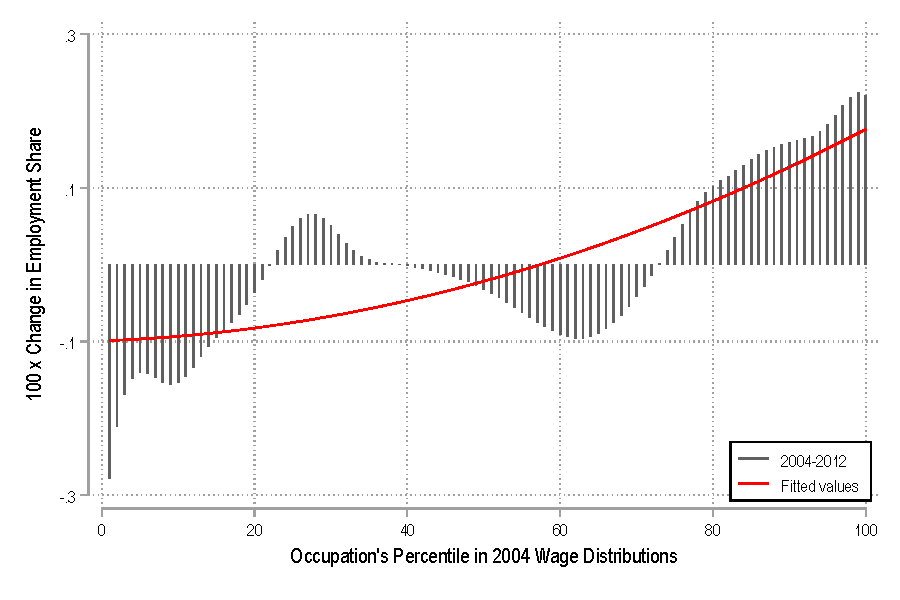
\includegraphics[width=0.5\textwidth]{figs/ch2/polarization-2004-2012.pdf}}\subfloat[\label{fig:Observed-Changes-(2004-2012)}Observed Changes (2004-2012)]{\centering{}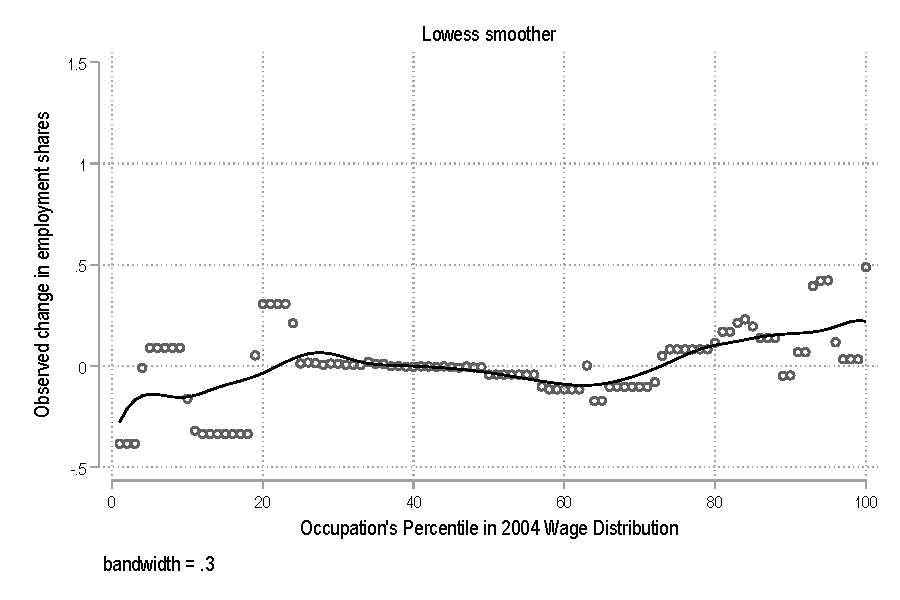
\includegraphics[width=0.5\textwidth]{figs/ch2/lowess-2004-2012.pdf}}
\par\end{centering}
\begin{centering}
\subfloat[\label{fig:Smoothed-Changes-(2012-2022)}Smoothed Changes (2012-2022)]{\centering{}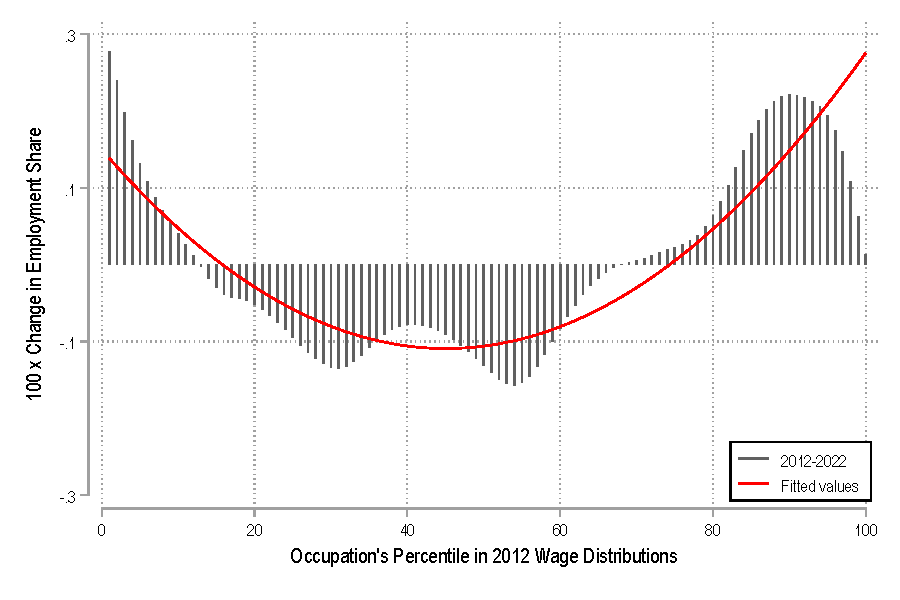
\includegraphics[width=0.5\textwidth]{figs/ch2/polarization-2012-2022.pdf}}\subfloat[\label{fig:Observed-Changes-(2012-2022)}Observed Changes (2012-2022)]{\centering{}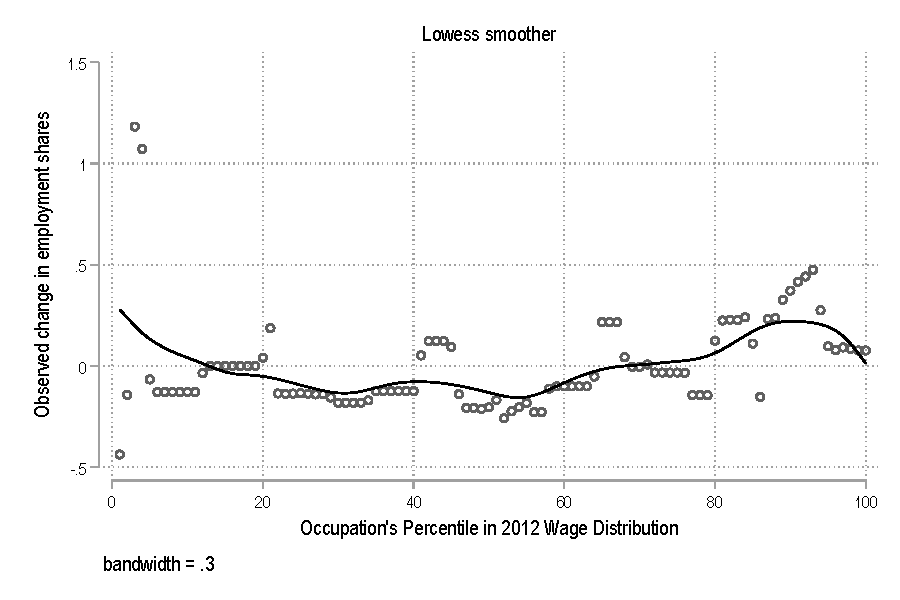
\includegraphics[width=0.5\textwidth]{figs/ch2/lowess-2012-2022.pdf}}
\par\end{centering}
\begin{centering}
\subfloat[\label{fig:Smoothed-Changes-(2004-2022)}Smoothed Changes (2004-2022)]{\centering{}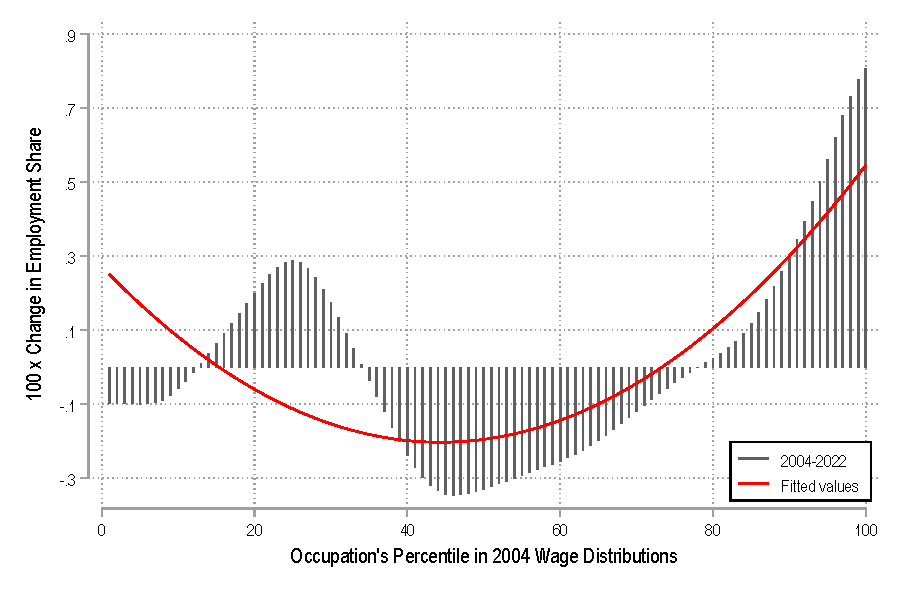
\includegraphics[width=0.5\textwidth]{figs/ch2/polarization-2004-2022.pdf}}\subfloat[\label{fig:Observed-Changes-(2004-2022)}Observed Changes (2004-2022)]{\centering{}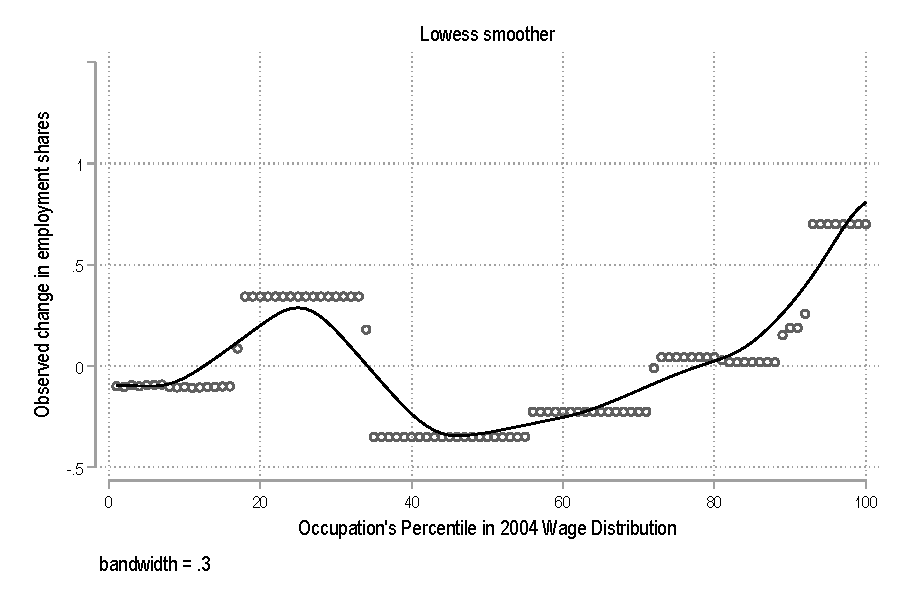
\includegraphics[width=0.5\textwidth]{figs/ch2/lowess-2004-2022.pdf}}
\par\end{centering}
\medskip

\textbf{Source:} Author's calculations using 2004, 2012 and 2022 waves
of HLFS. A smoothing regression (bw: 0.3) applied to follow the trend.
\end{figure}
\par\end{center}

\vspace{-1cm}

\begin{onehalfspace}
As the structural transformation is so evident, it allows us to distinguish
the percentiles associated with service occupations from those linked
with manufacturing occupations by observing the points above and below
the zero line. Notably, the 5 percentile points emerging after the
40th percentile correspond to cleaners and helpers (ISCO 91), exhibiting
a moderate growth rate. Conversely, the two deciles before and after
ISCO 91 are positioned below zero line and corresponds to occupations
within the manufacturing sector.

The situation is less clear in the first decile as depicted in Figure
\ref{fig:Observed-Changes-(2012-2022)}. Excluding the first and fifth
percentiles, all the intervening percentiles are associated with personal
service workers (ISCO 51 and ISCO 53) and sales workers (ISCO 52).
Notably, personal care workers (ISCO 53), constituting a two percent
of employment, experienced an extraordinary growth rate of over 100\%.
In contrast, jobs such as travel attendants, cooks, waiters, and hairdressers
(classified as ISCO 51) observed a decline in employment share, dropping
from 6.6\% to 5.5\%. Meanwhile, the employment share of sales jobs
remained steady at their 2012 level.

From Figure \ref{fig:Smoothed-Changes-(2004-2022)} and Figure \ref{fig:Observed-Changes-(2004-2022)},
we can track the general pattern of transformation in employment over
the past two decades. Similar to the first period, starting from around
the 40th percentiles, a monotonic trend emerges. Manufacturing jobs
(ISCO 7 and ISCO 8) experienced a substantial decline of 12\% in total
employment share, a trend that is visually apparent from the diminishing
employment between the 40th and 80th percentiles. The portion of employment
previously held by the manufacturing sector jobs has been redistributed
between occupations situated at the upper tail of the wage distribution,
in particular, managers and professionals, in conjunction with service
jobs concentrated around the 20th percentiles.
\end{onehalfspace}

\subsection{Calculating Task Contents}

\begin{onehalfspace}
In the first part of this subsection, We'll introduce a summary index
of routine task activities. Following \citet{2013Autor,2006Autor},
by averaging the scores of non-routine cognitive tasks we aggregate
them into an abstract task category. In addition to that, by averaging
the scores of routine tasks we created a routine task category. Finally,
by synthesizing these three task categories we obtain a composite
measure of routine task intensity RTI for each occupation, which has
the formal representation as follows
\begin{eqnarray}
RTI & = & ln(T_{kt}^{R})-ln(T_{kt}^{A})-ln(T_{kt}^{M}),\label{eq:RTI}
\end{eqnarray}

Whereby, $T_{kt}^{R}$, $T_{kt}^{A}$ and $T_{kt}^{M}$ are, respectively,
inputs of routine, abstract and manual task for each occupation \emph{$k$}
and year \emph{$t$.} Our summary measure RTI exhibits a positive
correlation with the prominence of routine tasks within an occupation,
while displaying a negative correlation with the prevalence of abstract
and manual tasks within the same occupation.
\end{onehalfspace}
\begin{center}
\begin{table}[H]
\caption{\label{tab:Summary_task_intensities}Task Intensity of Major Occupations
Categories}

\begin{centering}
\begin{tabular}{l>{\centering}p{1cm}>{\centering}p{2cm}>{\centering}p{2cm}>{\centering}p{2cm}}
\toprule 
 & \emph{RTI }index & Abstract tasks & Routine tasks & Manual tasks\tabularnewline
\cmidrule{2-5} \cmidrule{3-5} \cmidrule{4-5} \cmidrule{5-5} 
Managers/Legislators & - & \cellcolor[gray]{0.75}+ & - & -\tabularnewline
Professionals & - & \cellcolor[gray]{0.75}+ & - & -\tabularnewline
Technicians & - & \cellcolor[gray]{0.75}+ & - & -\tabularnewline
Clerks & + & - & \cellcolor[gray]{0.75}+ & -\tabularnewline
Service and sales & + & \cellcolor[gray]{0.75}+ & - & -\tabularnewline
Craft and related trade & - & - & + & \cellcolor[gray]{0.75}+\tabularnewline
Machine operators & + & - & \cellcolor[gray]{0.75}+ & +\tabularnewline
Elementary occupations & + & - & + & \cellcolor[gray]{0.75}+\tabularnewline
\bottomrule
\end{tabular}
\par\end{centering}
\medskip

\textbf{Notes:}The table constructed by following the work of \citet{2013Autor}.
The plus sign indicates that the average value of particular task
for that major occupation category is greater than the average. Minus
sings indicates that the opposite. Gray shaded boxes are signs of
that particular occupations' dominant task intensity.
\end{table}

\par\end{center}

\vspace{-1cm}

\begin{onehalfspace}
In table \ref{tab:Summary_task_intensities} we summarized average
task intensities of major occupational categories (agricultural workers
are excluded). Whit this exercise, we can elaborate on general occupational
task dimensions. As we going down the skill distribution, routine
intensities are increasing except for the construction workers who
are grouped under craft and related trade category, and manual tasks
are becoming more dominant.

To make a more detailed comparison between routine task intensities
and skill levels, we followed \citet{2013Autor} and separated occupations
according to their place in the routine index distribution and defined
the occupations in the top 1/3 as routine intensive. As we can see
from figure \ref{fig:Share-of-Routine}, the share of routine jobs
are the lowest at 1st percentile and after 80th percentile. Comparing
this with Figure \ref{fig:Smoothed-Change-(2004-2012)} which plots
the employment growth of skill percentiles between 2004 and 2012,
yields very interesting results. In each quintile of skills, if there
is a rise in routine occupation share, there is a decline in employment
share, and vice versa. The visual inspection of routine employment
shares reveals correspondence with Figure \ref{fig:Smoothed-Changes-(2012-2022)},
which plots the second period's employment growths. Between 20th and
60th percentiles in \ref{fig:Smoothed-Changes-(2012-2022)}, employment
decline matches to the increase in routine employment share in Figure
\ref{fig:Share-of-Routine}. The categorization of routine employment
share and more detailed statistics are displayed in Appendix Table
\ref{tab:Occupation's-Rank-by-RTI}.
\end{onehalfspace}
\begin{center}
\begin{figure}[H]
\caption{\label{fig:Share-of-Routine}Share of Routine Occupations by Occupational
Skill Percentile}

\begin{centering}
\noindent\resizebox{\textwidth}{!}{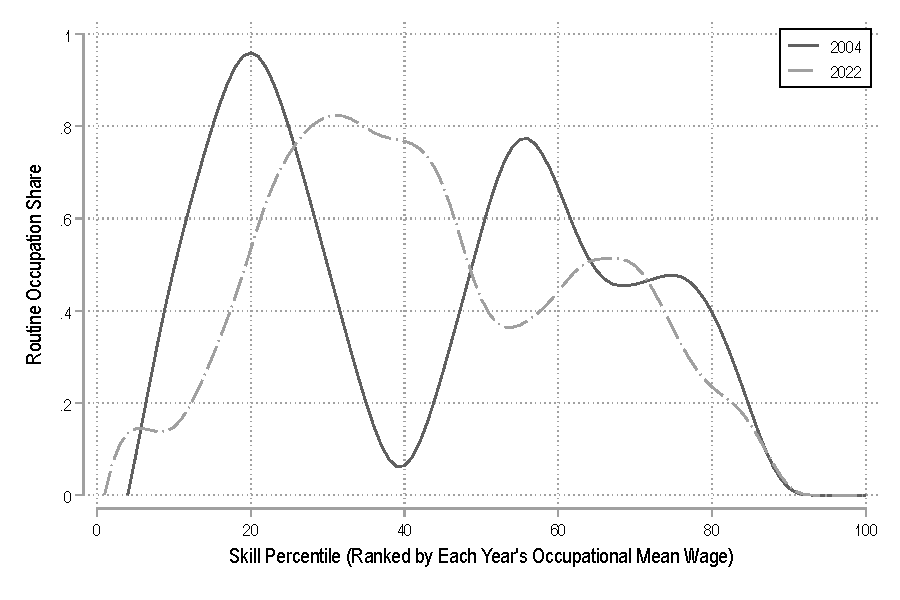
\includegraphics{figs/ch2/routine-occupation-share-2004-2022.pdf}}
\par\end{centering}
\medskip

\textbf{Notes: }To allow time variation in task measures, we used
waves of O{*}NET data corresponding to each year (O{*}NET 7.0 for
2004, and O{*}NET 17.0 for 2012). Also we use ISCO88 occupational
coding scheme for the year 2004, and ISCO08 occupational codings for
the year 2012. The allocation of occupations into percentiles was
predicated on their respective positions within the wage distribution
for each corresponding year. Applying an exclusion criteria similar
to Figure \ref{fig:Smoothed-Changes-in-Wages-and-Employment-2}, the
data was subjected to refinement, yielding resilient metrics for occupational
alignment across wage percentiles. Specifically, individuals such
as farmers and workers without available wage information during the
survey month have been excluded. Mean wage levels for each occupation
category was used to determine the order of occupations in percentiles.
Furthermore, we applied a smoothing regression with a bandwidth level
of 0.3, aiming to present a visually coherent representation of the
overarching trend. 
\end{figure}
\par\end{center}

\begin{center}
\begin{table}[H]
\begin{onehalfspace}
\caption{\label{tab:Means-and-standard}Means and standard deviations of O{*}NET
task measures for four broad occupational groups in 2015}

\begin{longtable}[c]{>{\raggedright}p{4cm}>{\centering}p{3cm}>{\centering}p{3cm}>{\centering}p{3cm}}
 & \textbf{\pbox{14cm}{Professional, \\ Managerial, \\ Technical}} & \textbf{\pbox{14cm}{Clerical, \\ Sales}} & \textbf{\pbox{14cm}{Production, \\ Operators, \\ Elementary}}\tabularnewline
\toprule & \multicolumn{3}{c}{Males and females combined}\tabularnewline
\midrule\rowgroup{Non-routine cognitive} &  &  & \tabularnewline
\pbox{12cm}{Non-routine cognitive \\ analytical} & 1.59 & -0.23 & -0.58\tabularnewline
\pbox{12cm}{Non-routine cognitive \\ personal} & 1.22 & 0.15 & -0.71\tabularnewline
\rowgroup{Non-routine manual} &  &  & \tabularnewline
\pbox{12cm}{Non-routine manual \\ physical} & -1.05 & -0.56 & 0.92\tabularnewline
\pbox{12cm}{Non-routine manual \\ personal} & 1.10 & 0.51 & -0.92\tabularnewline
\rowgroup{Routine} &  &  & \tabularnewline
Routine cognitive & -0.57 & 0.31 & 0.08\tabularnewline
Routine manual & -1.08 & -0.60 & 0.97\tabularnewline
\rowgroup{Routine task intensity} & -1.33 & 0.15 & 0.55\tabularnewline
\bottomrule
\end{longtable}\textbf{Source: }Author's calculations based on the methodology described
above.
\end{onehalfspace}
\end{table}

\par\end{center}

\vspace{-1cm}

\begin{onehalfspace}
In Table \ref{tab:Means-and-standard}, first three major occupational
categories are intensive in non-routine analytical and interpersonal
tasks such as solving problems, reading and news and professional
journals, supervising and giving speeches to others. Workers in Clerical
and Sales occupations (ISCO 4-5) are performing tasks which on average,
have more routine intensity than high skill workers. However, there
is a substantial difference in routine intensity of these middle skills
occupations. While clerical workers are attained to tasks with high
routine cognitive intensity, such as book keeping or calculating,
sales and service workers are doing non-routine cognitive and non-routine
manual personal tasks which requires advanced interpersonal relationship
skills.

Workers in occupations coded at the lower end of occupational distribution
are distinctly related to routine and manual tasks which have the
highest routine task intensity. Tasks in elementary occupations are
substantially higher in routine intensity and lack of cognitive elements.
\end{onehalfspace}
\begin{center}
\pagebreak
\par\end{center}

\begin{onehalfspace}
In order to analyze employment by task intensities, we allocate each
job a composite task measure, using the 2004 LFS and 2004 O{*}NET
as a reference point. Given that each occupation has multiple dimensions
concerning task requirements, it is imperative to establish a rule-based
decision-making framework to accurately allocate a task to each occupation.
Adopting from \citet{2018Fonseca} we allocate each occupation to
a task for which the occupation ranks highest in intensity. To present
formally, let each occupation $j$ in task $m$ have their rank denoted
as $rank_{jm}$. Occupation $j$ is considered to be more intensive
in task $m$ if $rank_{jm}>$ rank $rank_{ik}$, where $k\neq j$.
We applied the procedure for each occupation separately by utilizing
a simple sorting algorithm with a few exceptions. Agricultural occupations
are excluded, since their shares in services and manufacturing would
potentially be misleading to interpret. Additionally, managers of
small enterprises are excluded from the sample for two primary reasons.
Firstly, their employment share exhibited a continuous rise until
the occupational coding transition in 2012, followed by a nearly 5\%
decline with the introduction of the new coding scheme. Secondly,
the reported weekly working hours and wages for this subgroup are
notably distinct from the sample average, introducing incompatibilities.
Furthermore, observations associated with ISCO 33 were omitted due
to their limited representation, resulting from an insufficient number
of observation. The results are presented in Table \ref{tab:Allocation-Between-Occupations-and-tasks}.

Since tracking the employment share of each occupation beyond 2012
is not feasible, we adopted a similar methodology as described earlier,
but with 2012 as the base period, utilizing the 2012 LFS and O{*}NET
dataset. Nevertheless, another challenge arises from pooling two data
periods when aiming to analyze the complete sample period, stemming
from the abrupt change that occurred in 2012, as elaborated in the
data section. Our approach to address this concern involves a partially
compromising the observed values in 2012. Given the lack of comprehensive
information for 2012, apart from two variables indicating ISCO08 and
ISCO88 codes for each occupation, we computed employment changes for
the two periods separately using distinct occupational classifications.
Subsequently, we merged the outcomes by calculating the average of
the two samples for 2012. This approach enabled us to achieve a more
gradual transition between the two periods, albeit at the cost of
giving up the observed values for 2012.

Using the above procedure, we predicted trends in employment shares
by selected task for the economy, manufacturing and services. Note
that we include agricultural workers and construction workers in the
economy. Depicted in Figure \ref{fig:Employment-and-Tasks-1} approximately
half of the workers classified under the manual category for both
the services and the entire economy. Notably, the manual task proportion
witnessed a reduction of 10\% in the services sector and 5\% in the
economy.In spite of manual jobs, routine manual jobs are more prevalent
in the manufacturing sector. When combined with manual jobs, their
collective representation accounts for almost 80\% of the manufacturing
sector's workforce.

Furthermore, within both the manufacturing and services sectors, the
share of routine cognitive tasks reaches around 18\% in 2008, followed
by a nearly monotonic subsequent decline over the sample period. In
contrast, the trend for routine manual jobs in manufacturing and manual
jobs in services follows an opposing trajectory.
\end{onehalfspace}
\begin{onehalfspace}
\begin{center}
\begin{figure}[H]
\begin{centering}
\caption{Employment and Wage Changes by Task and Sector (2004-2022)}
\subfloat[\label{fig:Employment-and-Tasks-1}Employment Changes by Sector (2004-2022)]{\begin{centering}
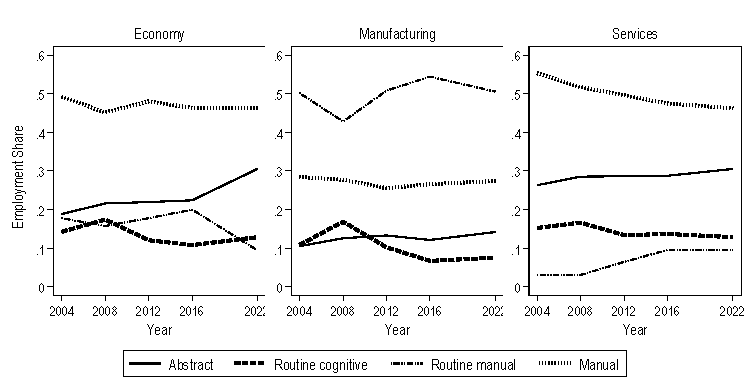
\includegraphics[width=1\textwidth]{figs/ch2/employment-by-task-sector.pdf}
\par\end{centering}
}
\par\end{centering}
\begin{centering}
\subfloat[\label{fig:Wages-and-Tasks-1-1}Real Wage Changes by Sector (2004-2022)]{\begin{centering}
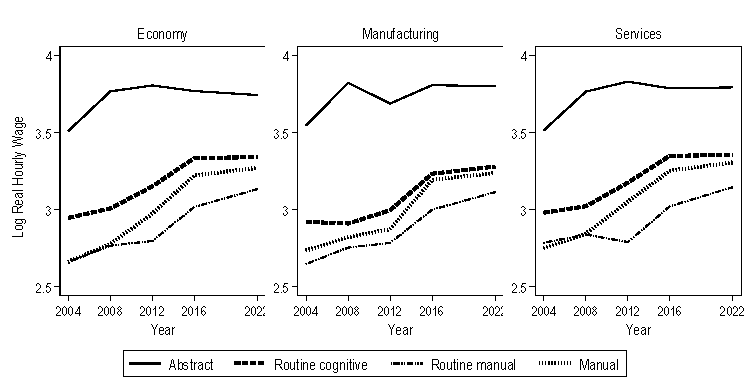
\includegraphics[width=1\textwidth]{figs/ch2/wages-by-task-sector.pdf}
\par\end{centering}
}
\par\end{centering}
\medskip

\textbf{Notes: }Employing a slightly altered framework compared to
Figure \ref{fig:Share-of-Routine}, we harnessed two waves of O{*}NET
data (O{*}NET 7.0 for 2004, O{*}NET 17.0 for 2012) to derive task
measures. Subsequent to the independent integration of standardized
task measures into the 2004 and 2012 datasets, we assigned each occupation
to a composite task measure for which the occupation ranks highest
in intensity. By aggregating each occupation's labor share to the
occupation's principal task component, we constructed a dataset comprising
employment shares for each task measure. Thus, this approach allows
us to trace the employment share of each composite task measure by
simply connecting each wave of data (2004, 2008, 2012, 2016 and 2022)
by using their occupational employment shares.
\end{figure}
\par\end{center}
\end{onehalfspace}

\begin{onehalfspace}
While in Figure \ref{fig:Employment-and-Tasks-1}, we can observe
an ascending trend in the category of abstract tasks, as reflected
in the relative shares of employment. However, the trajectories for
the remaining task categories, do not exhibit a consistent monotonic
pattern. In terms of log real weekly mean wages, an interesting pattern
emerges. In accordance with Figure \ref{fig:Smoothed-Changes-in-Wages-and-Employment-2}
and Figure \ref{fig:Composition-Adjusted-Educ-Cohorts-1},jobs characterized
by a significant intensity of cognitive element, displayed no real
wage growth after 2016, whereas, jobs with manual task component underwent
a notable surge in real wage growth rates over the study period, plotted
in Figure \ref{fig:Wages-and-Tasks-1-1}.

Figure \ref{fig:Employment-by-6-task-categories}, plots a more detailed
version of Figure \ref{fig:Employment-and-Tasks-1}, by employing
a stacked area graph scheme to display relative shares of tasks summing
up to a total of 1. A striking pattern emerges from Figure \ref{fig:Employment-by-6-task-categories},
which divides abstract and manual tasks into their subcomponents.
The jobs with personal task component (Non-routine manual personal
and Non-routine personal) in total, were just above 20\% of total
economy, in terms of total hours worked in 2004. However, by the year
2022, this share has undergone a remarkable growth, leading it to
encompass 55\% of the total hours worked within the economy.
\end{onehalfspace}
\begin{center}
\begin{figure}[H]
\caption{\label{fig:Employment-by-6-task-categories}Employment by 6 Task Categories
for All Sectors (2004-2022)}

\begin{centering}
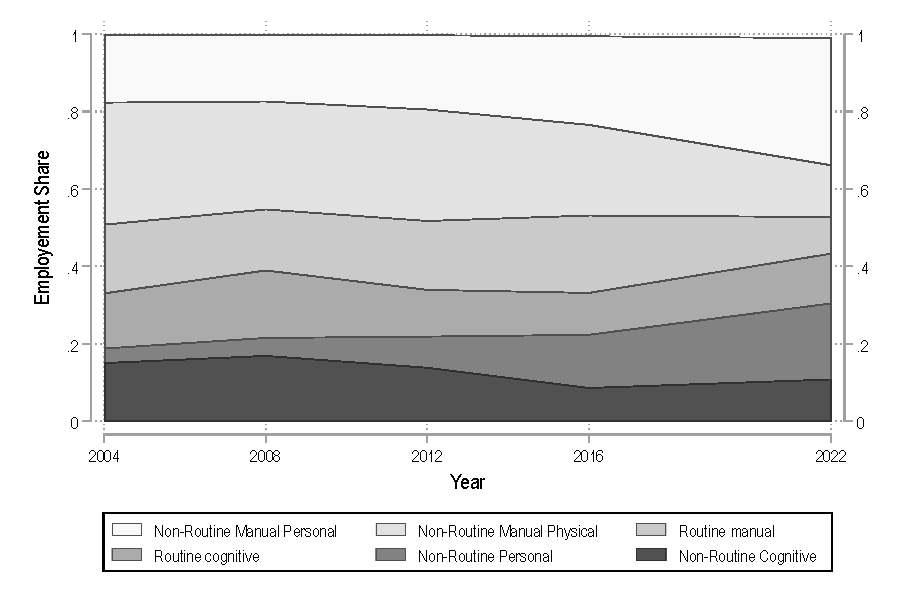
\includegraphics{figs/ch2/allsectors-alltasks-2004-2022-area.pdf}
\par\end{centering}
\medskip

\textbf{Notes: }Author's calculations based on O{*}NET data and corresponding
waves of HLFS.
\end{figure}
\par\end{center}

\begin{onehalfspace}
So far, our analysis has centered around task content data from occupations
in the United States, which aligns with the predominant approach taken
by numerous studies scrutinizing the US labor market \citep{2003Autor,2006Autor,2006SpitzOener,Acemoglu2011,2013Autor,2011Firpo},
as well as similar researches in Europe \citep{2007Goos,2009Goos,2014Goos,2018Hardy,2016Hardy,2018Fonseca,Aedo2013}.
The task content data used in these studies is sourced from two primary
databases: the Dictionary of Occupational Titles (DOT), which dates
back to 1939, and the Occupational Information Network (O{*}NET),
initiated in 2003. Both of these databases provides comprehensive
and periodically updated information regarding the specific tasks
linked to the occupations within the United States. Unfortunately,
no comparably comprehensive dataset has been systematically collected
for labor markets in other countries. As a result, studies examining
non-US labor markets often utilize the US task database and rely heavily
on the assumption of task content equivalence across different countries.

Aiming to account for country specific task content of occupations,
we adopted the methodology described in \citet{lewandowski2022,2020Rica}
in order to develop a task content metric specific to Turkey's labor
market by using the Programme for the International Assessment of
Adult Competencies (PIAAC) survey. Different from O{*}NET Data, this
survey comprises worker-specific information on daily tasks at work.
Moreover, the composite task measures are compatible with the well-established
job task measures used in \citet{Acemoglu2011}.

Our measure for non-routine cognitive analytical tasks incorporates
questions in PIAAC relating to problem-solving, reading news, engaging
with professional journals, solving problems, and programming. Meanwhile,
the measure for non-routine cognitive interpersonal tasks relies on
the activities such as supervising others and making presentations.
The routine cognitive task measure is based on sequentiality, where
the cognitive aspect stems from the ability to rearrange task order.
This is quantified by factors such as the inability to change the
order of tasks (reversed), form completion, and giving speeches or
presentations (reversed, denoting no speeches or presentations). To
compute the routine task intensity (RTI) using the PIAAC survey, we
apply the formula specified in equation \ref{eq:RTI}. In order to
prevent non-positive values in the logarithm, we add 1 for each task.The
occupation specific measures are provided in Figure \ref{fig:Country-Specific-Tasks}.
The table can be found in 

Analyzing the daily tasks that people undertake improved the understanding
of micro-level behaviors of workers to explain structural occupational
changes. Labor economists, collected information on workers' tasks
and used it for their analyses on the technology's role in explaining
job polarization, structural change and wage inequality. However,
this task-centric approach introduces its own set of challenges, most
prominently concerning the quantification and measurement of tasks.
Unlike skills, which can often be approximated using proxies such
as education or experience, tasks are intricately tied to the specific
requirements inherent to distinct occupations. Furthermore, the lack
of a universally accepted taxonomy for task classification compounds
the measurement challenge. Additionally, consistently collected data
sources across diverse labor markets are scarce, which further complicates
the task analysis landscape \citep{Biagi2020}. To illustrate the
issue, consider the case of ``non-routine manual'' major task category.
Across, various studies, this task category operationalized trough
different task components: ``hand-eye-foot coordination'' \citep{2013Autor},
(ii) ``time spent performing physical activities''
\citep{2013Autora}.

As pivotal contribution to the field, \citet{2003Autor} introduced
a taxonomy major task categories based on two main axes: Routine vs.
non-routine, and cognitive vs. manual. Subsequently, researchers such
as \citet{2013Autora,2013Autor} used a threefold classification:
Abstract, routine and manual. Threefold classification aggregates
non-routine tasks to obtain abstract tasks.

First we apply the methodology of \citet{Acemoglu2011} by using 3
O{*}NET data sets for 2004, 2012 and 2022 to obtain 5 major task categories
from 16 subset of tasks which are presented in Table \ref{tab:Construction-of-task}.
Nonetheless, while utilizing varied datasets enhances our capacity
to capture temporal shifts in task intensity across occupations, there
are two major shortcomings. Firstly, each wave of the O{*}NET dataset
focuses on the U.S. labor market and lacks dimensions specific to
labor markets of different countries. Secondly, the O{*}NET dataset
is constructed through the lens of experts who assign task values
based on the requisites of particular occupations. This expert-driven
perspective potentially introduces bias, as it lacks the workers'
perspective on their occupations \citep{Aedo2013}.

By using the methodology above, we create a data set, in which each
occupation \emph{$i$} is defined by a vector of tasks, \emph{$X_{ik}$,
}for the year $k$, and each occupation \emph{$i$} has a task intensity
value for each of the five skills which are not exclusive. The structure
is shown in the below matri
\[
X_{ik}=\left[\begin{array}{c}
X_{ik}^{Non-Routine\,Cognitive/Analyrical}\\
X_{ik}^{Non-Routine\,Cognitive/Interpersonal}\\
X_{ik}^{Routine\,Cognitive}\\
X_{ik}^{Routine\,Manual}\\
X_{ik}^{Non-Routine\,Manual\,Physical}
\end{array}\right]
\]

\citet{2018Hardy} extended the ALM and AA task framework to encompass
Europe by leveraging O{*}NET and EU-LFS data. Following their application,
we identify a subset of five tasks from a set of sixteen distinct
task requirements available within the O{*}NET data. These are, non-routine
cognitive analytical, non-routine cognitive interpersonal, routine
cognitive, routine manual, and non-routine manual physical tasks.
To facilitate integration with out occupations dataset, we employed
the crosswalk provided by \citet{2018Hardy}. The formulation of each
composite task measure involved the summation of the 16 task items,
which subsequently underwent a standardization process to attain a
mean of 0 and a standard deviation of 1. After having assigned each
task item $t$ to the LFS data, we apply a standardization procedure
to achieve comparability over time, and between each composite task
measure, following AA. The standardization process adheres to the
following formula:
\begin{eqnarray}
\forall i\forall j\in J & t_{i,j}^{std} & =\dfrac{t_{i}-\mu_{j}}{\delta_{j}},\label{eq:4}
\end{eqnarray}

\textbf{\textit{J}}, identifies the set of task items for \textbf{\textit{i}}
observation in the LFS which will be aggregated to obtain 5 composite
task measures mentioned above. $\mu_{j}$ is weighted average and
$\delta_{j}$ is the standard deviation of task item $j$. Weighted
average and standard deviation of each task item calculated with the
formulas below:
\begin{eqnarray}
\forall i\forall j\mu_{j} & = & \frac{\sum_{i=1}^{N}t_{i,j}w_{i}}{\sum_{i=1}^{N}w_{i}},\label{eq:mean}
\end{eqnarray}
\begin{eqnarray}
\forall i\forall j\delta_{j} & = & \left(\dfrac{\sum_{i=1}^{N}w_{i}(t_{i,j}-\mu_{j})}{\sum_{i=1}^{N}w_{i}}\right)^{1/2},\label{eq:standart_dev}
\end{eqnarray}

Whereby $w_{i}$ is the weight attributed to the observation \textbf{\textit{$i$}}
int he LFS dataset. Following the standardization of 16 task items,
we create 5 task measures by adding up the task items.
\end{onehalfspace}

\subsection{Estimation Strategy}

\setlength{\abovedisplayskip}{6pt} 

\setlength{\belowdisplayskip}{6pt}

\begin{onehalfspace}
The foundation for empirically analyzing the market's returns on investments
in human capital is rooted in the Mincer earnings model \citep{Mincer}.
Within this model, human capital is proxied by education and cumulative
experience. Notably, the coefficient associated with the duration
of schooling, as extracted from a logarithmic earnings regression,
is construed as the compensatory differential for the income foregone
during the years in education. If we assume unidimensional human capital
and competitive markets, the law of one price becomes applicable:
the comprehensive value of human capital should remain consistent
across various occupations. These presumptions can be shown in a hedonic
earnings model as the following:
\begin{eqnarray}
lnw_{i} & = & \alpha+\delta_{1}S_{i}+\delta_{2}\mathbf{X}_{i}+\delta_{3}Exp_{i}+\delta_{4}Exp_{i}^{2}+e_{i},\label{eq:mincermodel}
\end{eqnarray}

wherein, $w_{i}$ is the worker $i$'s log hourly wage, $\mathbf{X_{i}}$
is a vector of individual-level covariates, $S_{i}$ is years of educational
attainment, while the $Exp$, stands for the potential years of job
experience. The parameter $\hat{\delta_{i}}$ derived from the model
estimates of a market return associated with each year in school.
By incorporating the assumptions of negligible primary schooling costs
and the efficient functioning of the market, the model's predictions
indicate a convergence between the market interest rate and the equilibrium
return rate of each year in school. 

Can this model be extended to predict task prices using a wage regression
as in Eq. \ref{eq:mincermodel}? \citet{2013Autora} address this
inquiry by underscoring dissimilarities between tasks and education.
Firstly, the tasks are not durable investment goods contrary to education,
as the worker can modify task inputs according to a job's demands.
Consequently, this adaptive self-selection process negates the existence
of a direct correspondence between tasks and the human capital endowed
within workers. Secondly, unlike education, the tasks are a high-dimensional
bundle of activities in which the elements must be performed jointly
to produce output. 

To formally present the model of \citet{2013Autora}, let the worker
$i$ has a set of skill endowments $\Phi_{i}=\{\phi_{i1},\phi_{i2},...,\phi_{iK}\},$as
a vector of task efficiencies. Each element of vector $\Phi_{i}$
is a strictly positive number measuring the efficiency of a worker
$i$ at task $k$. Since the worker $i$ can perform $\phi_{iK}$
units of task $k$ in a given time interval, the $\Phi_{i}$ represents
the worker's human capital stock, and her productivity in producing
tasks is conditional on the human capital investments and the combination
of other abilities. 

Different from the standard Mincerian approach, the marginal productivity
of education is not equal across sectors. However, the productive
value of a task differs among occupations, which produce the output
using the vector of task K. Therefore, the output of a worker $i$
in occupation $j$ is as follows:
\[
Y_{ij}=e^{\alpha_{j}+\sum_{k}\lambda_{jk}\phi_{jk}+\mu_{i}},
\]

whereby $\lambda_{jk}$$\geq0$ $\forall$ $j,k$ and $\alpha_{j}$is
not strictly positive, since the marginal product of a worker's task
production would yield negative values conditional on the insufficiency
of skill endowments. If the workers wage is equal to her marginal
product, the log wage equation can be written as:
\[
w_{i}=\alpha_{j}+\sum_{k}\lambda_{jk}\phi_{jk}+\mu_{i},
\]

Within this production structure, if we allow for each worker to choose
their occupation to yield the most output, which maximizes her earnings,
her maximization problem will be as follows:
\[
Y_{i}=\underset{j}{max}\{Y_{i1},Y_{i2},...,Y_{iK},\}=\underset{j}{max}\{\alpha_{j}+\Phi_{i}\Lambda_{j}^{\prime}\},
\]

where $\Lambda_{j}$ is a vector denotes the production structure
of occupation $j$, $\Lambda_{j}=\{\alpha_{j},\lambda_{j1},\lambda_{j2},\allowbreak...,\lambda_{jk}\}$.
Within this model, the task returns are specific to occupation: $\partial w/\partial\phi_{k}\mid_{J=j}=\lambda_{jk}$. 

\citet{2013Autora} provides testable restrictions for their model
to identify structural parameters underlying this model. Next, we
summarize the two testable proposition and their specification for
empirically testing them. 
\end{onehalfspace}

\begin{theorem}

\begin{onehalfspace}
The covariance among task returns, and between task returns and the
constant term cannot be uniformly positive. 
\end{onehalfspace}

\end{theorem}

To test this implication, we conduct a series of estimations, as shown
in the following equation:
\begin{eqnarray}
W_{ij}=a_{j}+\delta_{jA}A_{i}+\delta_{jR}R_{i}+\delta_{jM}M_{i}+e_{ji},\label{eq:mincer12}
\end{eqnarray}

\begin{onehalfspace}
Where, the subscript ``j'' is indicative
of different occupations. We estimate the Eq. \ref{eq:mincer12} separately
for each occupation with a minimum of 5 observations, The resulting
estimated parameters from these regressions are preserved to form
a dataset. This dataset is then employed to perform bivariate regressions
among the components \{$a_{j}$, $\delta_{jA}$, $\delta_{jR}$, $\delta_{jM}$\},
with each regression being weighted by the employment size of the
respective occupation, as in the following: 
\begin{eqnarray}
\begin{array}{c}
\widehat{\delta_{jA}}=\alpha_{1}+\gamma_{1}\widehat{\delta_{jR}}+e_{12},\\
\\
\widehat{\alpha_{j}}=\alpha_{3}+\gamma_{3}\widehat{\delta_{jA}}+e_{01},
\end{array} & \begin{array}{c}
\widehat{\delta_{jA}}=\alpha_{2}+\gamma_{2}\widehat{\delta_{jM}}+e_{13},\\
\\
\widehat{\alpha_{j}}=\alpha_{4}+\gamma_{4}\widehat{\delta_{jR}}+e_{02},
\end{array} & \begin{array}{c}
\\
\\
\widehat{\alpha_{j}}=\alpha_{5}+\gamma_{5}\widehat{\delta_{jM}}+e_{03},
\end{array}\label{eq:bivariate-regressions}
\end{eqnarray}

\end{onehalfspace}

\begin{theorem}

\begin{onehalfspace}
To enable workers to positively self-select into occupation j based
on their proficiency in task 1 and into occupation j \textasciiacute{}
based on their proficiency in task 2, a fundamental requirement is
that:
\begin{eqnarray}
\rho & < & min\left(\dfrac{\lambda_{1}}{\lambda_{2}^{\prime}},\dfrac{\lambda_{2}^{\prime}}{\lambda_{1}}\right),\label{eq:self-selection}
\end{eqnarray}

Where $\rho\leq0,$ meaning that the workers abilities on different
tasks are either uncorrelated, or negatively correlated. 
\end{onehalfspace}

\end{theorem}

\begin{onehalfspace}
This proposition aligns the model with the principle of comparative
advantage, where individuals select occupations that best use of their
inherent strengths, leading to a more efficient allocation of labor
resources. Therefore, the self-selection implies non-zero covariances
between occupation-level task returns, and workers' endowments. To
capture these covariances, \citet{2013Autora} offers the following
specification, in which the average task measures of each occupation
interacted with the individual level task inputs: 
\begin{eqnarray}
\begin{array}{c}
W_{i}\\
\\
\\
\end{array} & \begin{array}{c}
=\\
\\
\\
\end{array} & \begin{array}{c}
a+\delta_{A}A_{i}+\delta_{R}R_{i}+\delta_{M}M_{i}+\beta_{A}\overline{A_{j}}+\beta_{R}\overline{R_{j}}+\beta_{M}\overline{M_{j}}\\
\\
+\gamma_{A}A_{i}\times\overline{A_{j}}+\gamma_{R}R_{i}\times\overline{R_{j}}+\gamma_{M}M_{i}\times\overline{M_{j}}\mathbf{+\theta X_{i}+\varepsilon_{i}}
\end{array}\label{eq:aheq10}
\end{eqnarray}

Most analyses on job tasks often conceptualize tasks as an occupational
level construct. However, a notable advantage offered by the PIAAC
\citep{2016} micro dataset is its provision of individual-level measures.
This facilitates an exploration of the variability in job tasks within
specific occupations, as well as an examination of the extent to which
this variability is systematically associated with both worker-related
factors and job-specific attributes. In the next section, we empirically
test this model's implications.
\end{onehalfspace}

\newpage{}
